%
% User Guide for KOA (re)count application
%
% $Id$ 
%
\documentclass{article}

\usepackage{ifpdf}

\ifpdf
\usepackage[pdftex,bookmarks=false,
            plainpages=false,naturalnames=true,
            colorlinks=true,pdfstartview=FitV,
            linkcolor=blue,citecolor=blue,urlcolor=blue]{hyperref}
\else
\usepackage[dvips]{hyperref}
\fi

\usepackage{url}
\usepackage{xspace}
\usepackage{eurosym}

\usepackage[dutch]{babel}
\usepackage{graphicx}

\newcommand{\opnieuw}{Opnieuw Beginnen}
\newcommand{\wissen}{Wissen Gegevens}
\newcommand{\importkan}{Importeren Kandidatenbestand}
\newcommand{\importstem}{Importeren Export Stembus}
\newcommand{\importpriv}{Importeren Private Sleutel}
\newcommand{\importpub}{Importeren Publieke Sleutel}
\newcommand{\ontsleutel}{Ontsleutelen}
\newcommand{\tel}{Tellen}
\newcommand{\rapport}{Rapporteren}
\newcommand{\help}{Help}
\newcommand{\sluit}{Sluiten}
\newcommand{\meer}{Meer Info}
\newcommand{\minder}{Minder Info}
\newcommand{\ok}{OK}
\newcommand{\annuleren}{Annuleren}
\newcommand{\verwerking}{Verwerkingsverslag}
\newcommand{\resultaat}{Resultaat stemming}
\newcommand{\cancel}{Cancel}

\newcommand{\myhref}[2]{\ifpdf\href{#1}{#2}\else\texttt{#2}\fi}

\title{Gebruikershandleiding Hertelapplicatie Kiezen op Afstand}
\author{Security of Systems Groep\\Katholieke Universiteit Nijmegen}

% The next line is automatically updated by 'make release'.
% (Also called by 'make distr' and 'make src_distr'.)
% Hence do not edit manually!
\date{Release v2.0}%%%RELEASE

\addtocounter{topnumber}{10}
\addtocounter{bottomnumber}{10}
\addtocounter{totalnumber}{10}
\renewcommand{\topfraction}{.95}
\renewcommand{\bottomfraction}{.95}
\renewcommand{\textfraction}{.01}
\renewcommand{\floatsep}{0.0cm}
\renewcommand{\textfloatsep}{0.25cm}
\renewcommand{\intextsep}{0.25cm}
\begin{document}

\maketitle
\tableofcontents
\section{Toelichting}

Deze applicatie behelst een telsysteem voor elektronisch uitgebrachte stemmen.
Doel is om de uitvoer die door de programmatuur van LogicaCMG wordt gegenereerd,
te kunnen controleren. Vandaar de benaming `hertelapplicatie'. Uiteraard kan dit programma ook als gewoon telprogramma gebruikt worden om de uitslag van de
betreffende verkiezingen te bepalen.

Het programma is specifiek geschreven voor de Europese verkiezingen van 2004. Het kan echter zonder wijzigingen ook voor andere verkiezingen gebruikt worden.
\section{Installatie}
De totale distributie is een \texttt{.zip} file. Na uitpakken levert dit een subdirectory \texttt{koa}. Deze directory bevat de files \texttt{koa.jar}, \texttt{koa.sh} en \texttt{koa.bat}.
De eerste file bevat het echte programma. De andere twee files zijn scriptfiles
die de applicatie goed opstarten.

Onder Windows moet men \texttt{koa.bat} uitvoeren.
En onder Linux \texttt{koa.sh}.

Deze twee files kunnen overigens met een standaard editor aangepast worden om 
de prestaties van de hertelapplicatie te verbeteren.
In deze files wordt namelijk een parameter gebruikt die de maximale heapsize
voor Java aangeeft. Standaard staat deze ingesteld op 180Mb. Indien de applicatie meer dan 180Mb gebruikt, zal de garbage collector aan het werk worden gezet
om niet meer gebruikt geheugen vrij te geven.
Op een machine met 256Mb RAM betekent dit dat Java 180Mb mag gebruiken, zodat er
nog genoeg overblijft voor het operating system zelf.
Indien de machine meer geheugen heeft, kan deze parameter navenant aangepast
worden.

Uiteraard werkt dit alleen maar als ofwel de J2SE Java Runtime Environment (JRE) ofwel de J2SE Software Development Kit (SDK) op het systeem ge\"installeerd is.
Onze applicatie is gebaseerd op Java versie 1.4.2.
Zie \cite{JAVAurl}.

\section{Graphical User Interface}
De GUI is zeer simpel van opzet. Conform \cite{PVEBZK} bestaat het programma uit een serie knoppen die stapsgewijs tot de einduitslag van de verkiezingen zullen leiden.

Het programma dwingt af dat de verschillende functies alleen maar in de juiste volgorde kunnen worden uitgevoerd.

Zie figuur~\ref{fig:mainmenu} voor het hoofdmenu zoals dat eruitziet na het opstarten van het programma.
\begin{figure}[htb]
\begin{center}
\ifpdf
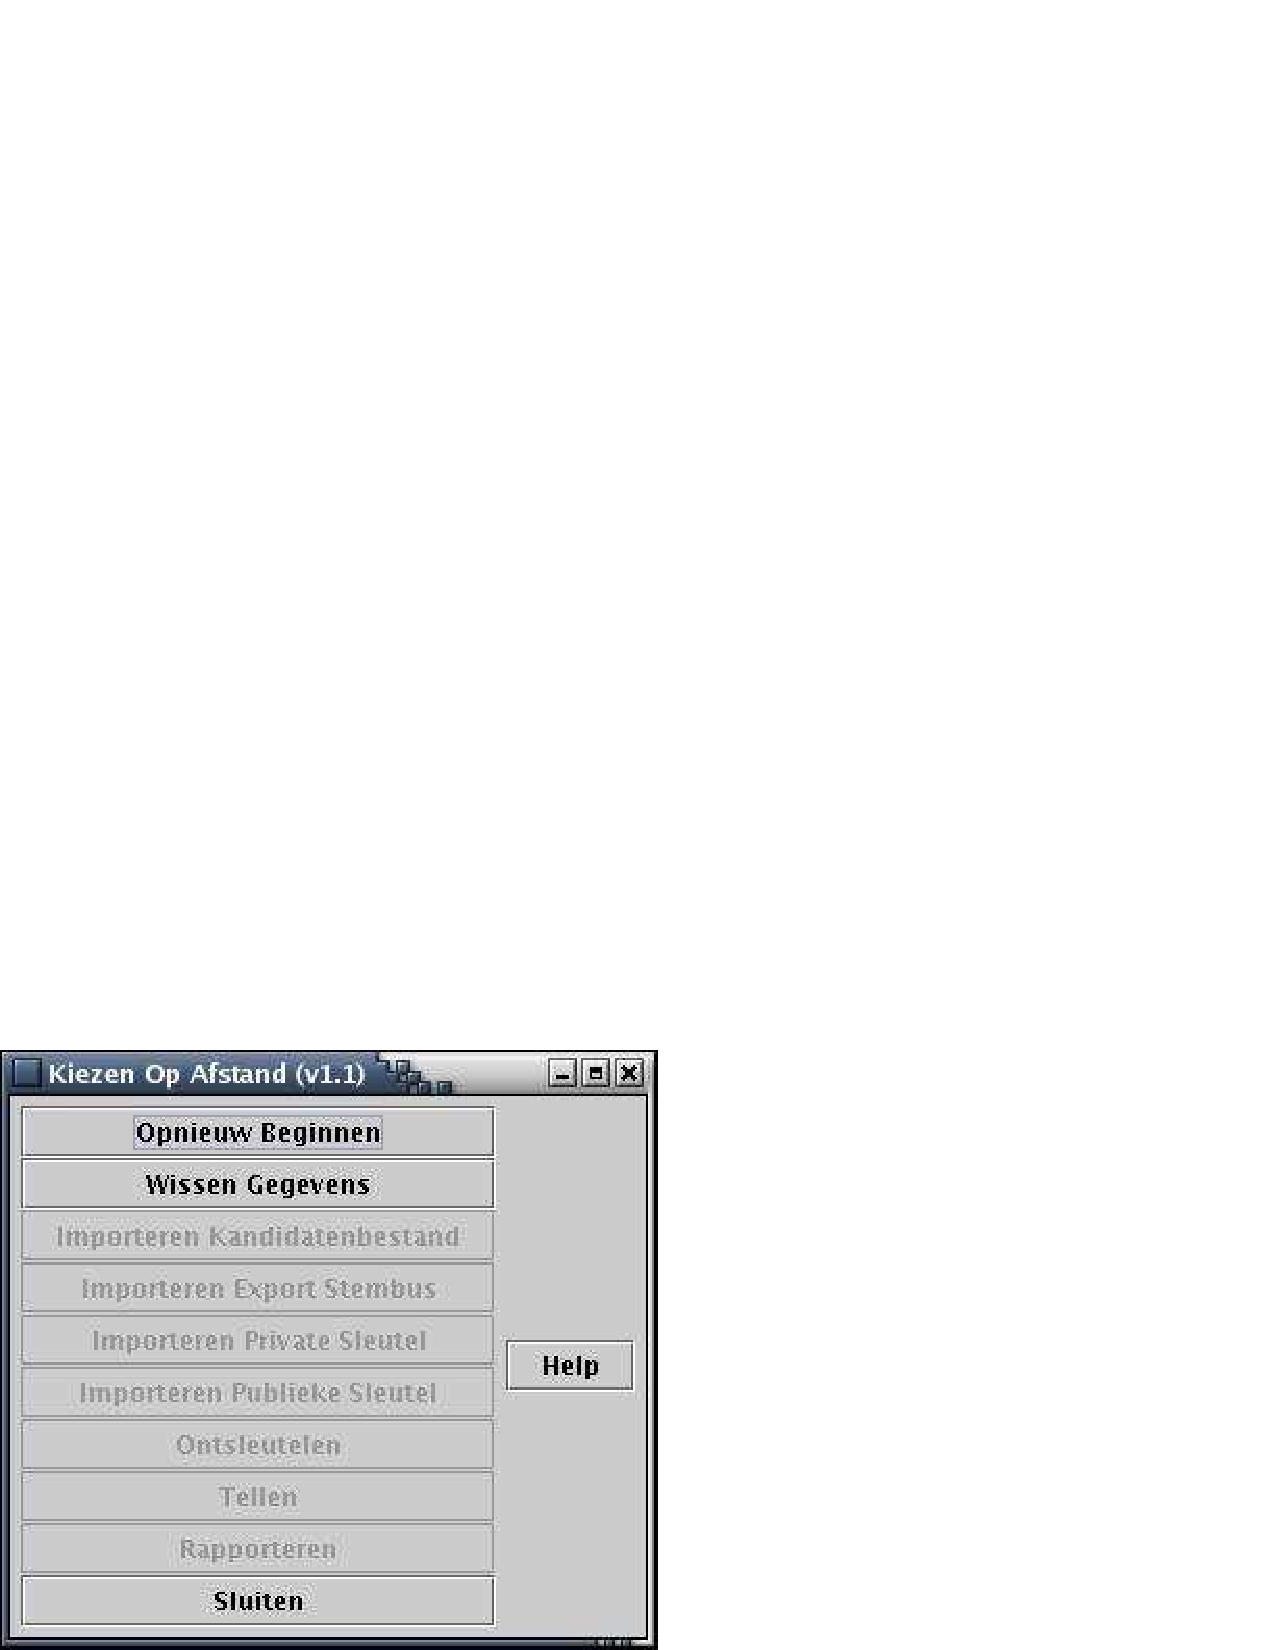
\includegraphics[scale=0.45]{scherm01}
\else
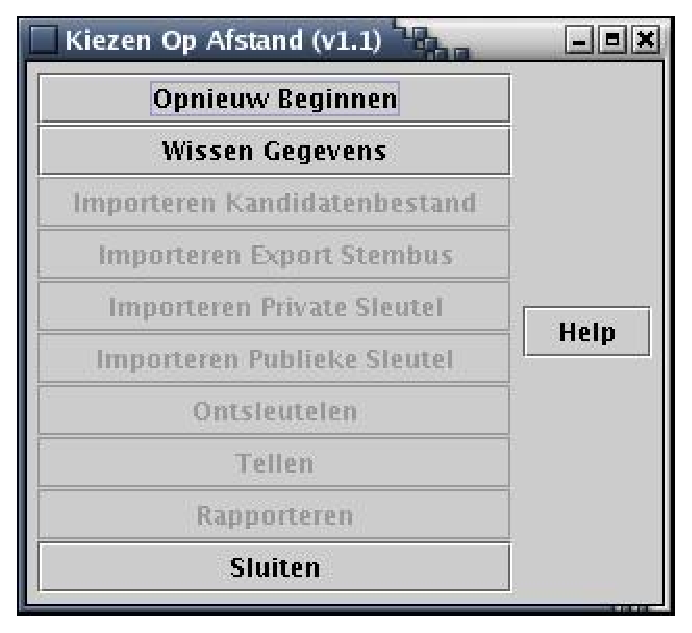
\includegraphics[scale=0.45]{scherm01.eps}
\fi
\caption{Hoofdmenu na opstarten}
\label{fig:mainmenu}
\end{center}
\end{figure}
De extra informatie wordt telkens via popup schermen aan de gebruiker getoond.
\section{Handleiding}
\subsection{\opnieuw}
Deze knop is toegevoegd om het mogelijk te maken om tijdens een sessie opnieuw te kunnen beginnen. Op het moment van indrukken wordt er overigens nog geen informatie gewist. Dat gebeurt pas bij het indrukken van `\wissen'. Deze functie is uiteraard altijd actief. Het is echter niet mogelijk om na het indrukken van deze knop nog bij de oude gegevens in het geheugen te kunnen. Men kan dan alleen nog gebruik maken van de rapporten die op de harde schijf zijn weggeschreven.
\subsection{\wissen}
Deze functie wist het interne geheugen en verwijdert eventuele rapporten die
als file zijn weggeschreven van de harde schijf. Voor dat er echt iets gewist wordt, moet de gebruiker eerst deze functie bevestigen in een dialoogscherm.
Als er files op de harde schijf staan worden deze files opgesomd in het dialoogscherm waar de gebruiker de bevestiging moet geven.
Zie figuur~\ref{fig:wis}.
\begin{figure}[htb]
\begin{center}
\ifpdf
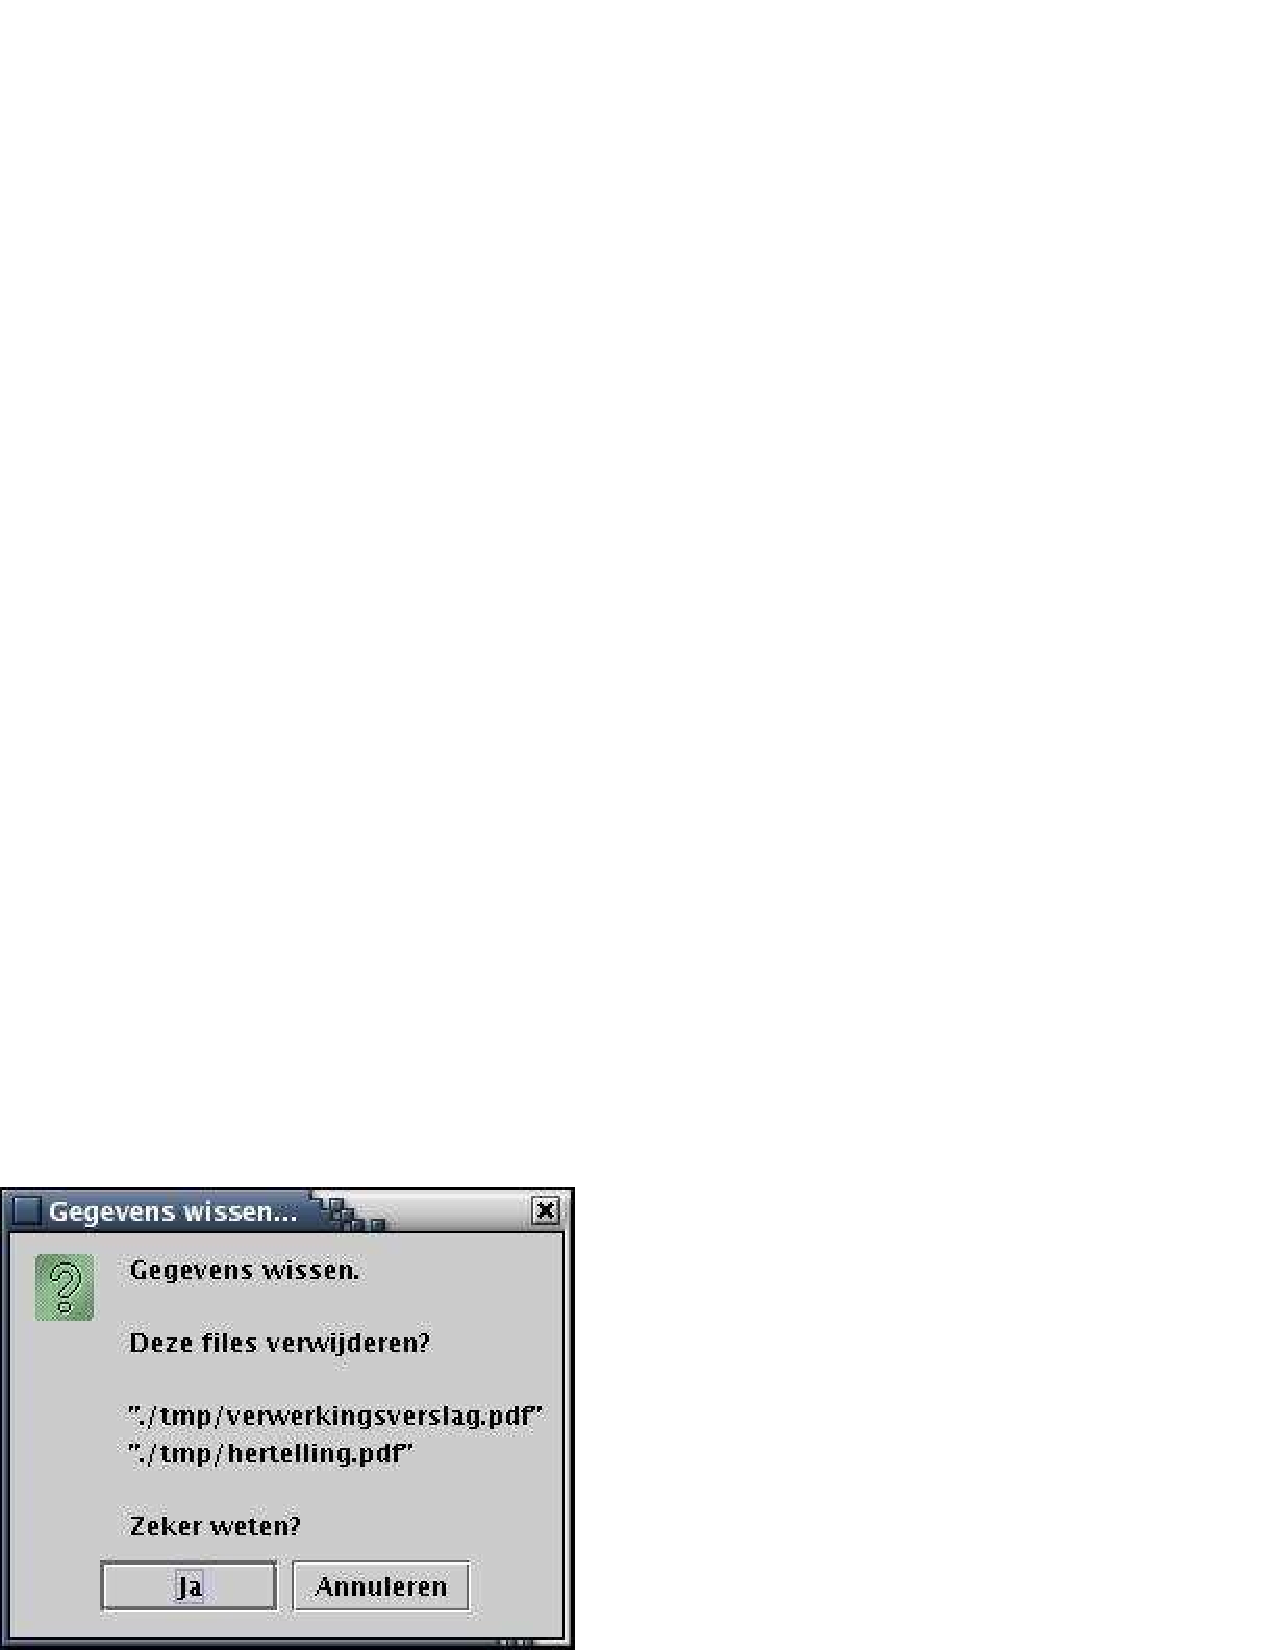
\includegraphics[scale=0.45]{scherm02}
\else

\includegraphics[scale=0.45]{scherm02.eps}
\fi
\caption{\wissen}
\label{fig:wis}
\end{center}
\end{figure}
Na bevestiging volgt een mededeling of het wissen gelukt is of niet.
%%Zie figuur~\ref{fig:wis2}.
%%\begin{figure}[htb]
%%\begin{center}
%%\ifpdf
%%
\includegraphics[scale=0.45]{scherm03}
%%\else
%%
\includegraphics[scale=0.45]{scherm03.eps}
%%\fi
%%\caption{Status \wissen}
%%\label{fig:wis2}
%%\end{center}
%%\end{figure}
\subsection{\importkan}
Er wordt een filebrowse scherm getoond waarin de gebruiker de gewenste XML file moet kiezen. Er wordt standaard een filter toegepast zodat er alleen maar files met \texttt{.xml} extensie worden getoond.

Aangezien dit een standaard component is, is dit scherm helaas in het Engels. Maar gezien het feit dat de functionaliteit zeer universeel is, mag dit geen probleem opleveren.
\begin{figure}[htb]
\begin{center}
\ifpdf
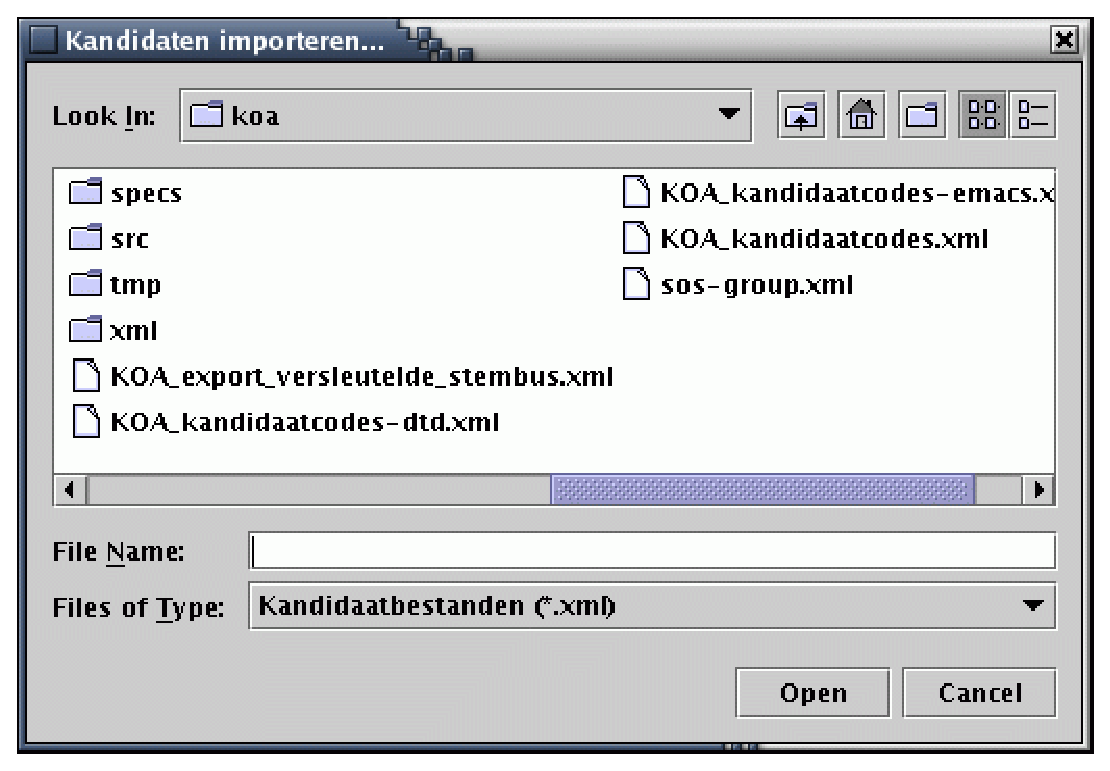
\includegraphics[scale=0.45]{scherm04}
\else
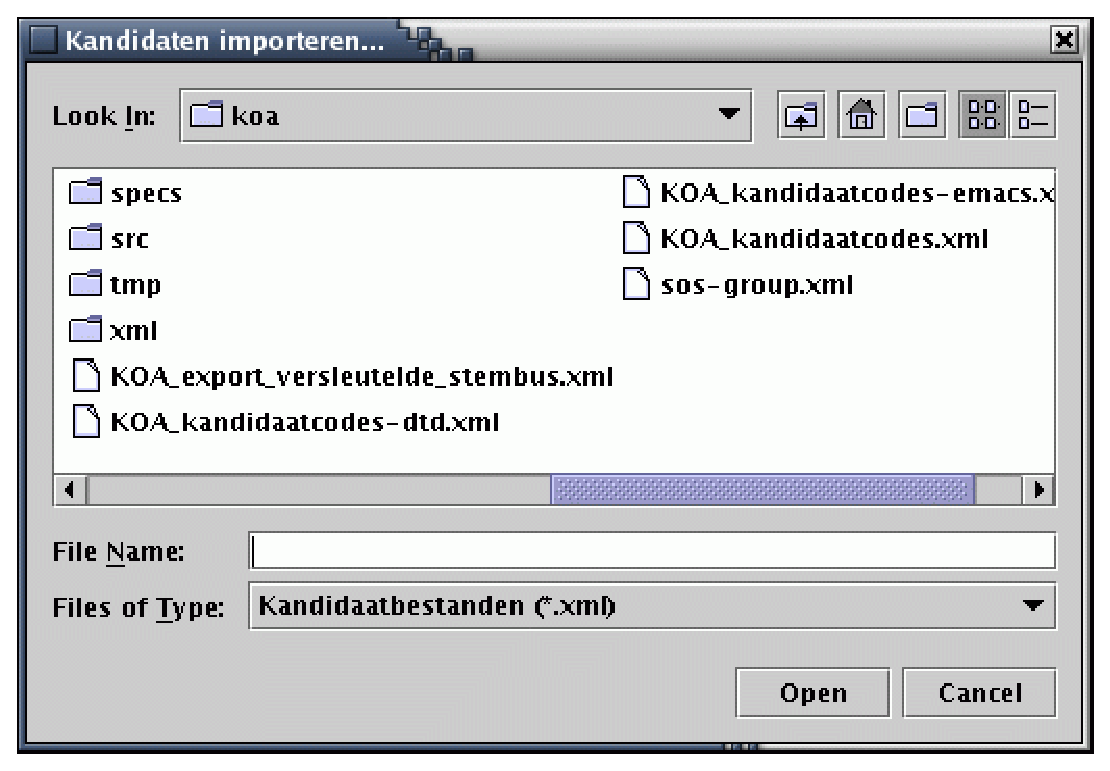
\includegraphics[scale=0.45]{scherm04.eps}
\fi
\caption{\importkan}
\label{fig:filebrowse}
\end{center}
\end{figure}

Na keuze van de file, wordt geprobeerd die file in te lezen.
Afhankelijk van de grootte van de file, zal er een voortgangsbalk tevoorschijn
komen. Op het moment dat op de daarbij getoonde `\cancel' gedrukt wordt, worden
de op dat moment reeds ingelezen gegevens gewist.

Als het opgegeven bestand niet van het juiste type is, zal er een foutmelding worden getoond.
Is het bestand wel een echt kandidatenbestand dan zal er een scherm getoond worden met daarin een overzicht van de gevonden kieskringen en kieslijsten. Per kieslijst wordt aangegeven hoeveel kandidaten er zijn gevonden.
Zie figuur~\ref{fig:importkan}.
\begin{figure}[htb]
\begin{center}
\ifpdf
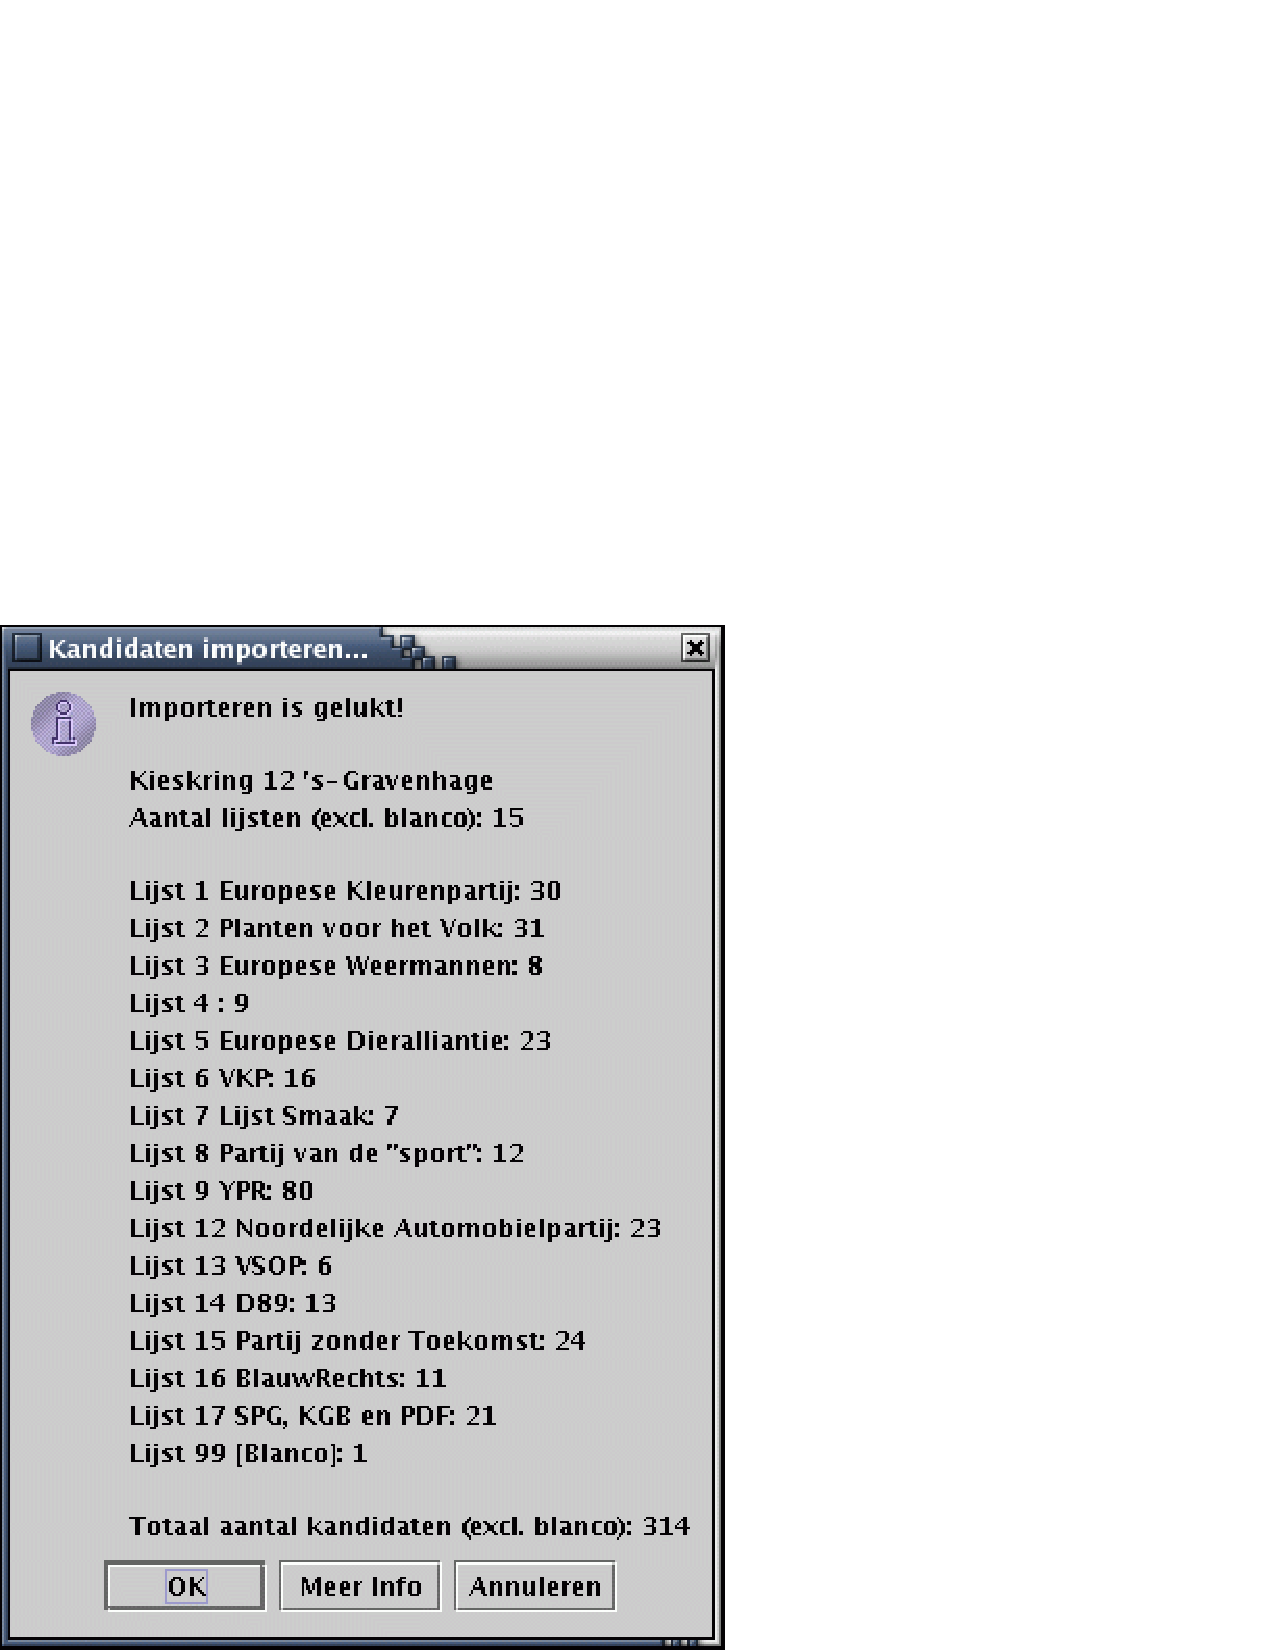
\includegraphics[scale=0.45]{scherm05}
\else
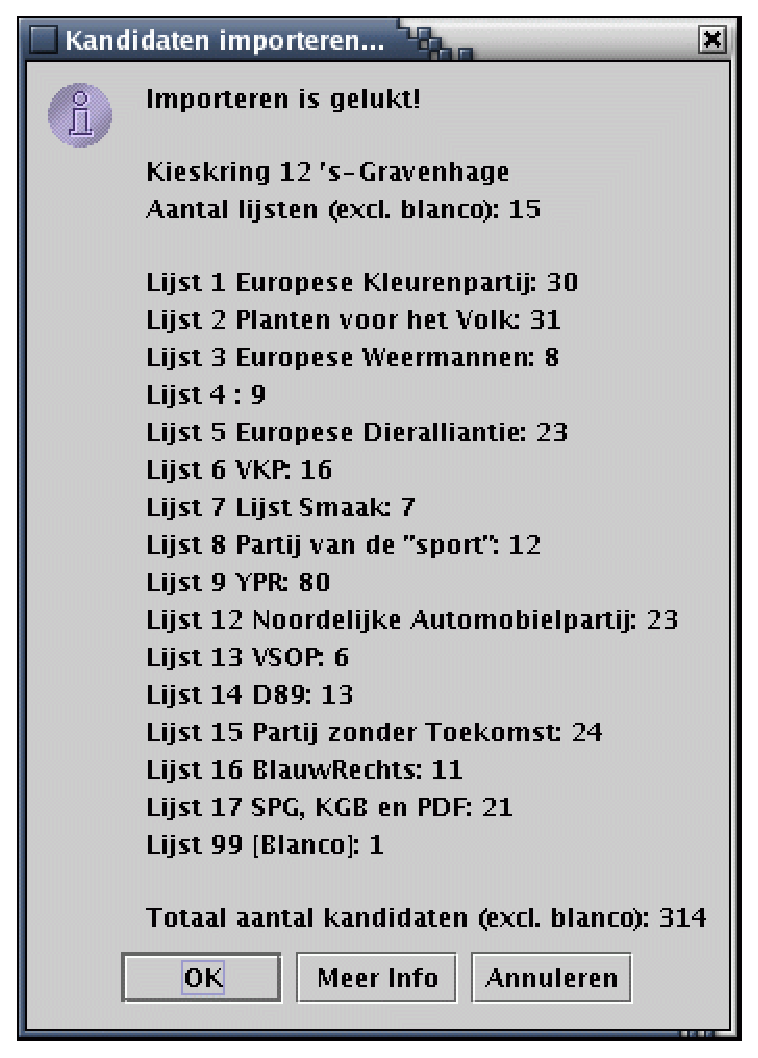
\includegraphics[scale=0.45]{scherm05.eps}
\fi
\caption{\importkan\ resultaat}
\label{fig:importkan}
\end{center}
\end{figure}

De knop `\ok' zorgt ervoor dat de gegevens geaccepteerd worden en dat er vervolgens een bestand met stemmen kan worden ingelezen.

De knop `\annuleren' zorgt ervoor dat de gegevens niet gebruikt worden. Te gebruiken als men per ongeluk een geldig maar verkeerd kandidatenbestand heeft ingelezen.

De knop `\meer' geeft de gebruiker een lijst te zien met alle kandidaten.
Is voor deze optie gekozen, kan men via `\minder' weer terug naar het vorige scherm. De knoppen `\ok' en `\annuleren' werken hetzelfde als in het scherm met de beperkte informatie.  Zie figuur~\ref{fig:meerinfo}.
\begin{figure}[htb]
\begin{center}
\ifpdf
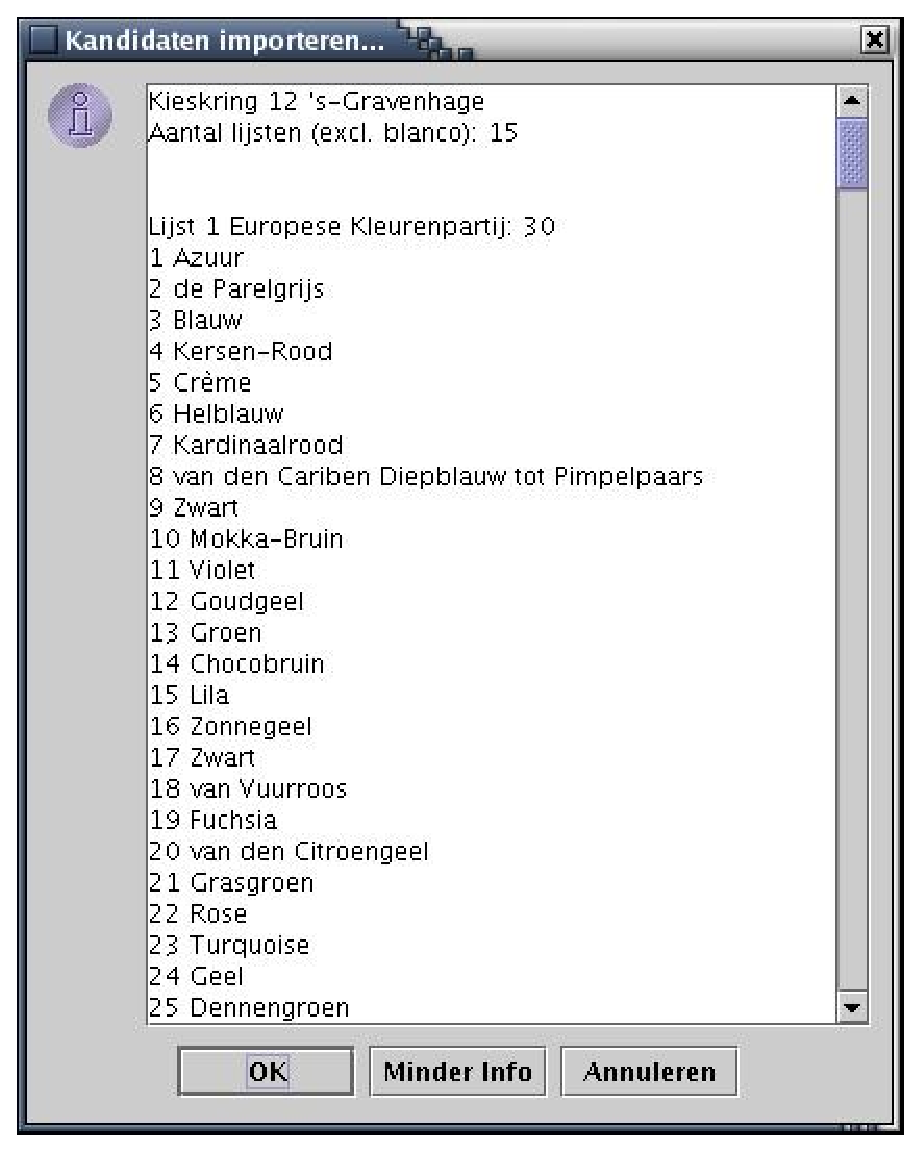
\includegraphics[scale=0.45]{scherm06}
\else
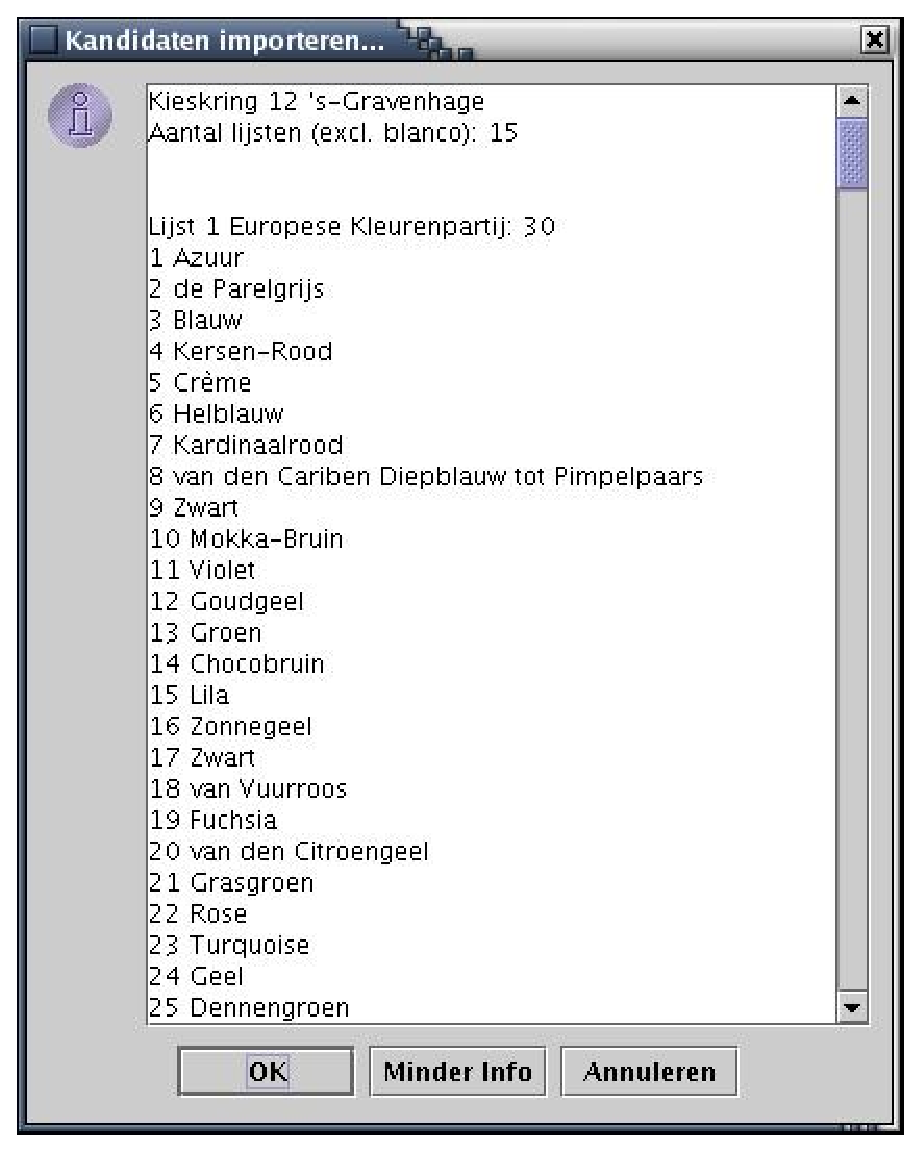
\includegraphics[scale=0.45]{scherm06.eps}
\fi
\caption{\meer}
\label{fig:meerinfo}
\end{center}
\end{figure}
\subsection{\importstem}
Ook nu wordt er een filebrowser geopend. Het filter staat weer op \texttt{.xml} ingesteld, maar er wordt wel duidelijk gemaakt dat het nu om stembusbestanden gaat.

Is de gekozen file van een ongeldig formaat, wordt er weer een foutmelding getoond. Is het wel een goede file wordt vervolgens een overzicht getoond waarin het aantal aangetroffen kieskringen en het aantal aangetroffen mogelijke stemmen wordt getoond. Zie figuur~\ref{fig:importstem}.
\begin{figure}[htb]
\begin{center}
\ifpdf

\includegraphics[scale=0.45]{scherm07}
\else

\includegraphics[scale=0.45]{scherm07.eps}
\fi
\caption{\importstem}
\label{fig:importstem}
\end{center}
\end{figure}

Ook hier kan weer via `\ok' danwel `\annuleren' door de gebruiker gekozen worden om deze gegevens te accepteren of niet.

Afhankelijk van het aantal in te lezen stemmen, kan deze actie erg lang duren.
Na enkele seconden verschijnt er dan ook een voortgangsbalk met daarbij de geschatte tijd die het nog duurt om deze actie af te ronden.
Zie figuur~\ref{fig:progress}.
Doordat deze tijd gebaseerd is op een schatting van de uit te voeren taak, is de informatie met name aan het begin niet altijd even nauwkeurig.
Wordt op de `\cancel' knop gedrukt, dan worden alle tot dan toe ingelezen stemmen
weggegooid.
\begin{figure}[htb]
\begin{center}
\ifpdf

\includegraphics[scale=0.45]{scherm21}
\else

\includegraphics[scale=0.45]{scherm21.eps}
\fi
\caption{\importstem\ voortgangsbalk}
\label{fig:progress}
\end{center}
\end{figure}
\subsection{\importpriv}
De getoonde filebrowser heeft het filter ingesteld op \texttt{.key} bestanden.
Na selectie van het bestand met de private sleutel, wordt de gebruiker gevraagd
om het bijbehorende wachtwoord te geven.
Zie figuur~\ref{fig:prive}.
\begin{figure}[htb]
\begin{center}
\ifpdf

\includegraphics[scale=0.45]{scherm08}
\else

\includegraphics[scale=0.45]{scherm08.eps}
\fi
\caption{\importpriv}
\label{fig:prive}
\end{center}
\end{figure}

De gebruiker krijgt een melding op het scherm of het inlezen van deze sleutel gelukt is of niet.

\subsection{\importpub}
Voor de gebruiker werkt dit hetzelfde als bij de private sleutel.
Op de achtergrond is er echter een verschil.
Na het kijken of het inlezen van deze publieke sleutel gelukt is, wordt een extra test gedaan om te bepalen of de private en publieke sleutel ook een zogenaamd
sleutelpaar vormen.
Is dat niet het geval dan wordt hier melding van gemaakt.
De gebruiker kan dan direct een nieuwe publieke sleutel inlezen.
Zat het probleem echter in de keuze van een verkeerde private sleutel, zit er
niets anders op dan de knop `\opnieuw' te gebruiken.
\begin{figure}[htb]
\begin{center}
\ifpdf

\includegraphics[scale=0.45]{scherm09}
\else

\includegraphics[scale=0.45]{scherm09.eps}
\fi
\caption{\importpub\ mislukt}
\label{fig:pub}
\end{center}
\end{figure}

In het bijzonder betekent de melding dat importeren gelukt is, dus automatisch ook dat er nu een geldig sleutelpaar is ingelezen. Zie figuur~\ref{fig:pub}.
\subsection{\ontsleutel}
Deze functie gebruikt de ingelezen sleutels om de ingelezen versleutelde stemmen te ontsleutelen.
Op het scherm wordt het aantal ontsleutelde stemmen getoond. Zie figuur~\ref{fig:ontsleutel}.
Dit kan kleiner zijn dan het aantal ingelezen stemmen als bij sommige stemmen de ontsleuteling mislukt is.
\begin{figure}[htb]
\begin{center}
\ifpdf
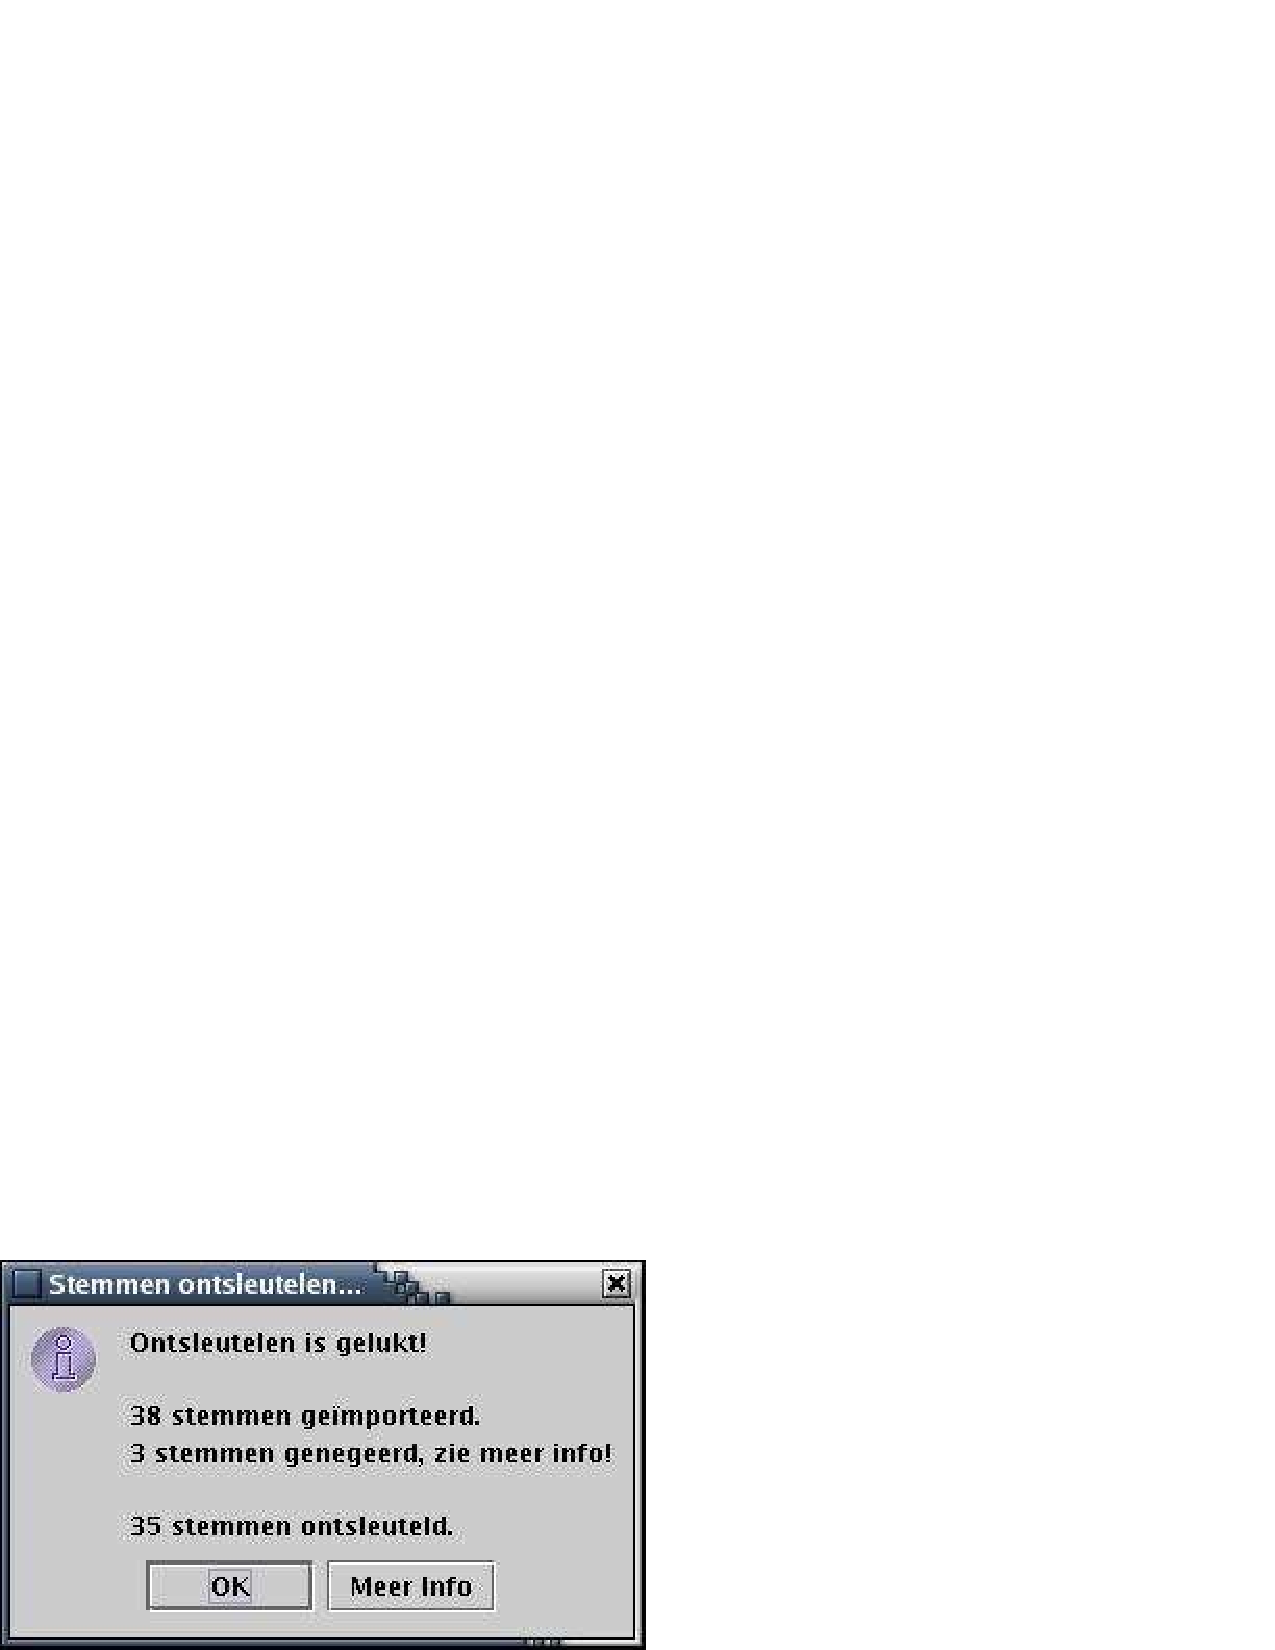
\includegraphics[scale=0.45]{scherm10}
\else

\includegraphics[scale=0.45]{scherm10.eps}
\fi
\caption{\ontsleutel}
\label{fig:ontsleutel}
\end{center}
\end{figure}
De knop `\meer' toont de eventuele problemen per stem. Zie figuur~\ref{fig:ontsleutelprob}.
\begin{figure}[htb]
\begin{center}
\ifpdf
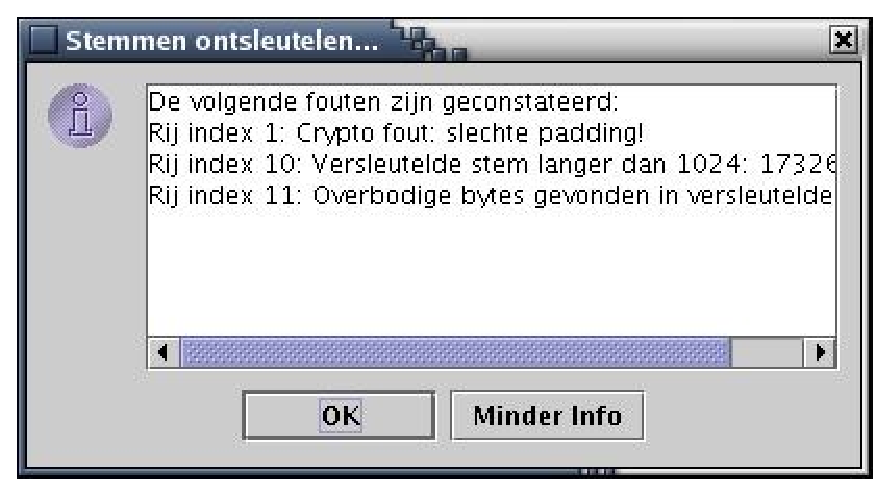
\includegraphics[scale=0.45]{scherm22}
\else
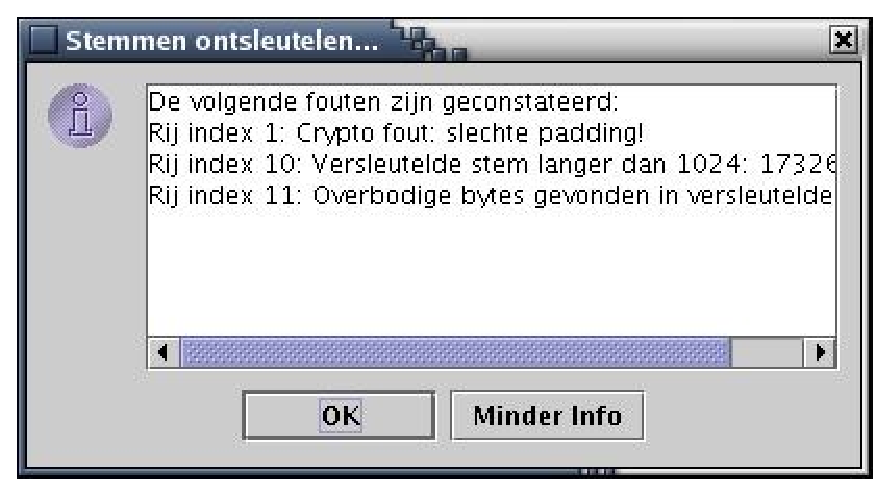
\includegraphics[scale=0.45]{scherm22.eps}
\fi
\caption{\ontsleutel\ foutmeldingen}
\label{fig:ontsleutelprob}
\end{center}
\end{figure}

Deze functie kan niet geannuleerd worden. In het bijzonder betekent dit dat de
`\cancel' optie die onder de voortgangsbalk staat geen echte annulering
inhoudt.
Bij een volgende poging tot ontsleutelen worden de inmiddels ontsleutelde 
stemmen uit de vorige run overgeslagen en direct geteld als reeds ontsleuteld.
Wat dat betreft is deze `\cancel' meer een onderbreking dan een annulering.
Echter een zij-effect is dat eventuele foutmeldingen bij het ontsleutelen
worden gewist. 

Er wordt een file \texttt{tmp/decrypted.txt} aangemaakt met daarin de ontsleutelde stemmen. 
Elke stem staat op een aparte regel.
Als dit allemaal geldige stemmen zijn, zullen de verschillende velden van 
elkaar gescheiden zijn door een `;'. Op het moment dat er iets anders dan een
geldige stem tevoorschijn is gekomen uit de ontsleuteling, is er niets te 
zeggen over de inhoud van zo'n regel.

\subsection{\tel}
Deze functie telt de ontsleutelde stemmen.
Aan de hand van de kandidaatcode in de stem, wordt een kandidaat gezocht in de lijst met kandidaten. Vervolgens wordt de redundante informatie in de stem vergeleken met de informatie die bij die kandidaat hoort. Verder wordt gecontroleerd of de kieskring correct is.
\begin{figure}[htb]
\begin{center}
\ifpdf

\includegraphics[scale=0.45]{scherm11}
\else

\includegraphics[scale=0.45]{scherm11.eps}
\fi
\caption{\tel}
\label{fig:tel}
\end{center}
\end{figure}
Wordt deze validatie doorstaan, dan zal het aantal uitgebrachte stemmen voor deze kandidaat met \'e\'en opgehoogd worden.
Gaat er iets mis met deze validatie wordt er niets gedaan met deze stem en gaat het programma gewoon verder met de volgende stem.

Na afloop wordt het aantal stemmen dat geldig was getoond.  Zie figuur~\ref{fig:tel}.
De knop `\meer' toont weer de eventuele problemen per stem. Zie figuur~\ref{fig:telprob}. Merk hierbij op dat rijen waarbij de ontsleuteling al mislukt was, er nu niet opnieuw geprobeerd is om deze stemmen te tellen en er hier dus ook geen foutmelding over die rijen te zien is.
\begin{figure}[htb]
\begin{center}
\ifpdf

\includegraphics[scale=0.45]{scherm23}
\else

\includegraphics[scale=0.45]{scherm23.eps}
\fi
\caption{\tel\ foutmeldingen}
\label{fig:telprob}
\end{center}
\end{figure}

Als het tellen eenmaal is afgerond, kan deze functie niet meer geannuleerd
worden. Als het tellen echter zo lang duurt dat er een voortgangsbalk 
verschijnt, kan via de dan ook getoonde '\cancel' knop de actie wel
onderbroken worden. Door de vastgelegde toestandsovergangen, betekent dat
echter alleen dat de gebruiker verder weinig keus heeft: ofwel kan er opnieuw
geteld worden met dezelfde invoer, ofwel kan er helemaal opnieuw begonnen
worden, ofwel kan het programma afgesloten worden.
In elk geval is het zo dat bij elke keer dat het tellen opnieuw wordt gestart,
alle tellers bij de kandidaten en partijen weer op 0 worden gezet.


\subsection{\rapport}
Deze functie biedt de gebruiker een popup scherm met daarin de keuze tussen
`\verwerking' danwel `\resultaat' en `\annuleren'. Zie figuur~\ref{fig:rapport1}.
\begin{figure}[htb]
\begin{center}
\ifpdf

\includegraphics[scale=0.45]{scherm12}
\else

\includegraphics[scale=0.45]{scherm12.eps}
\fi
\caption{\rapport}
\label{fig:rapport1}
\end{center}
\end{figure}

Voor `\verwerking' zijn inmiddels alle gegevens bekend. Vandaar dat de machinerie automatisch aan het werk gaat. Als het goed is komt er een melding dat het verslag is aangemaakt en is weggeschreven op de harde schijf. Indien de applicatie er in slaagt een PDF viewer te vinden op het systeem, zal die automatisch gestart worden om dit verslag op het scherm te tonen.
\begin{figure}[htb]
\begin{center}
\ifpdf

\includegraphics[scale=0.45]{scherm13}
\else

\includegraphics[scale=0.45]{scherm13.eps}
\fi
\caption{\rapport\ resultaat}
\label{fig:rapport2}
\end{center}
\end{figure}

\begin{figure}[htb]
\begin{center}
\ifpdf
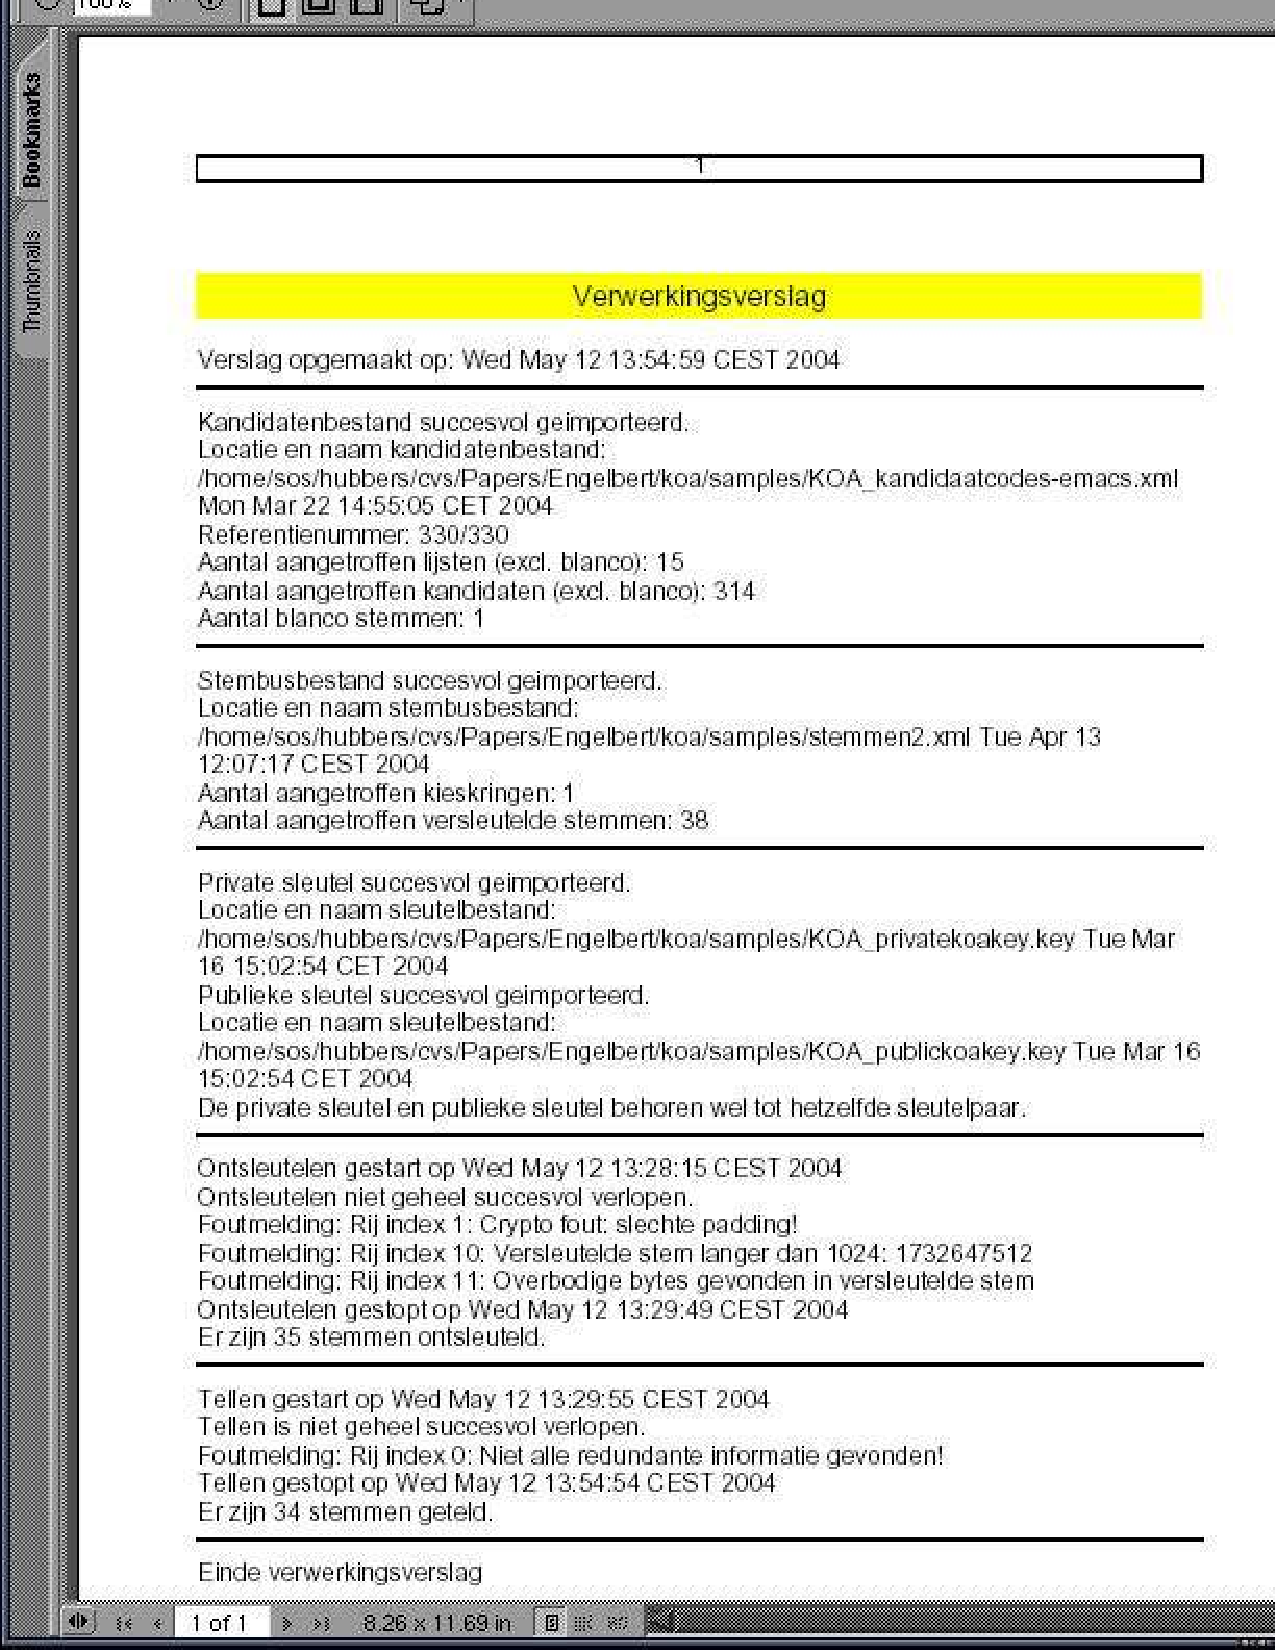
\includegraphics[scale=0.45]{scherm18}
\else
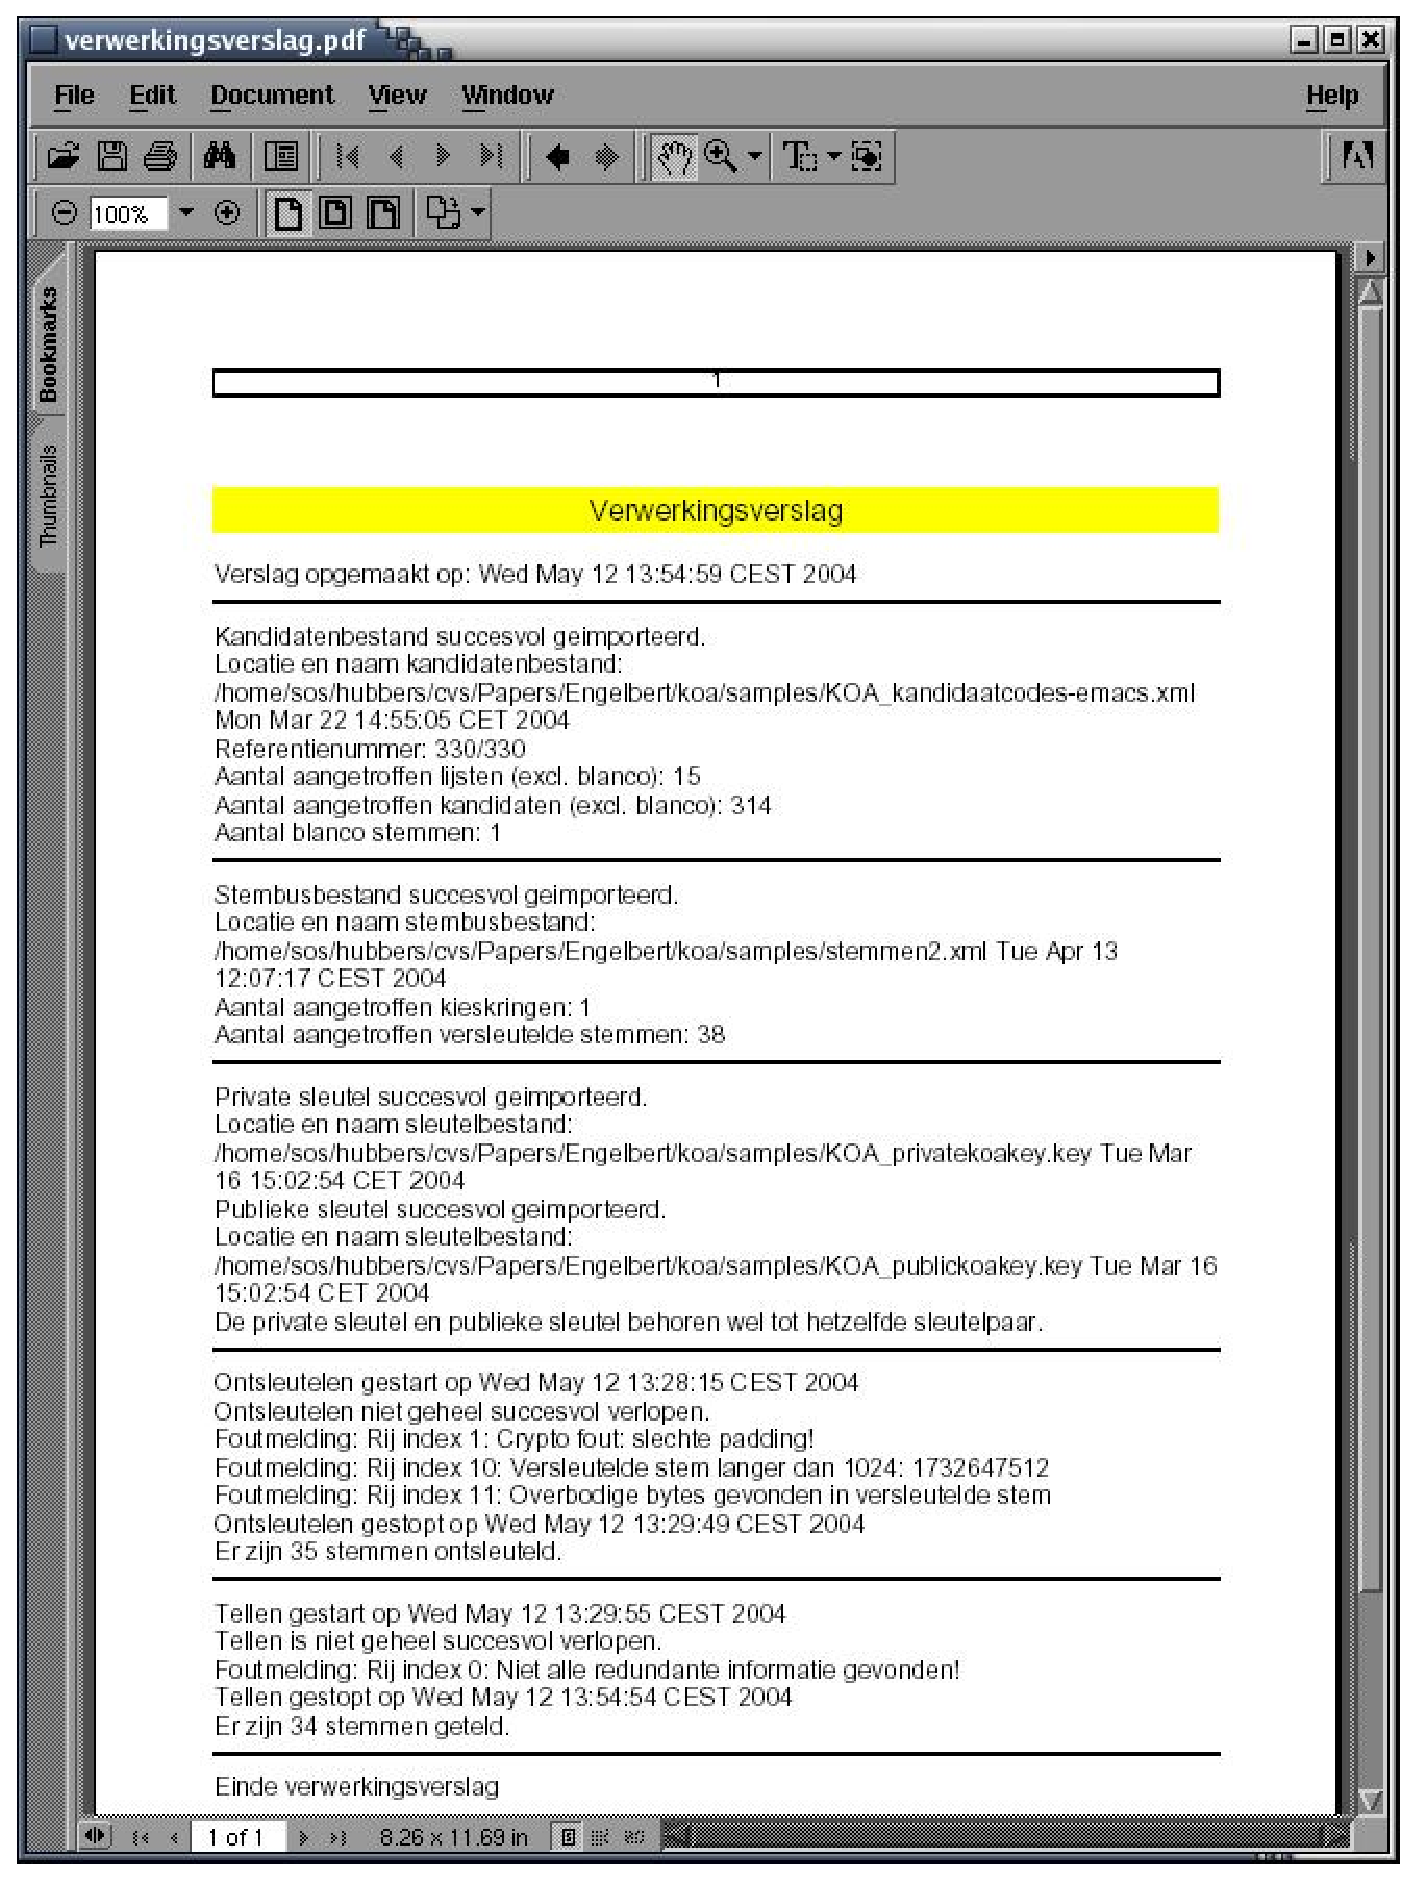
\includegraphics[scale=0.45]{scherm18.eps}
\fi
\caption{\rapport\ \verwerking}
\label{fig:rapport3}
\end{center}
\end{figure}

Merk op dat in figuur~\ref{fig:rapport3} bij het ontsleutelen en het tellen de foutmeldingen per stem worden getoond.

Voor `\resultaat' zijn nog niet alle gegevens bekend en daarom komen er nog twee popup schermen langs.
Bij het eerste scherm (figuur~\ref{fig:rapport4}) wordt de gebruiker gevraagd om de stemperiode te geven. Standaard wordt hier de periode specifiek voor de Europese verkiezingen van 2004 genoemd.
\begin{figure}[htb]
\begin{center}
\ifpdf
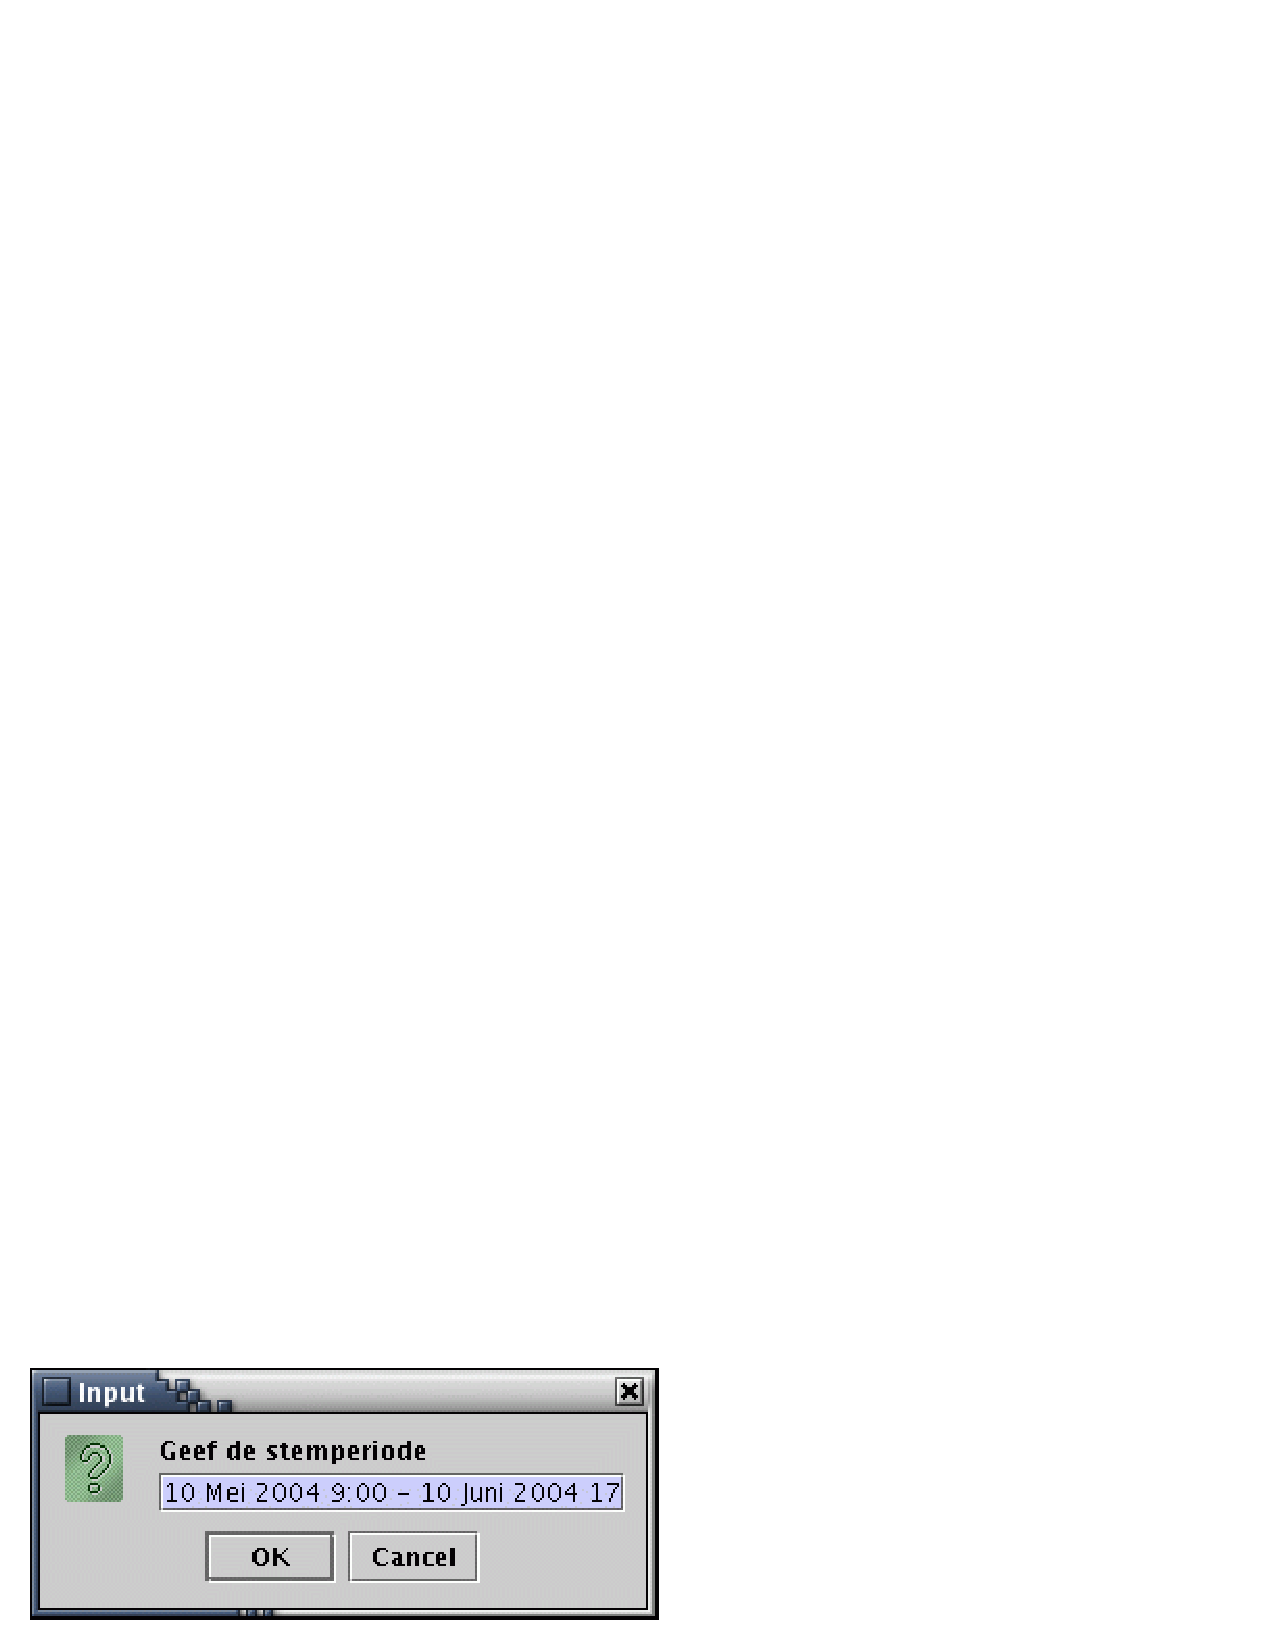
\includegraphics[scale=0.45]{scherm14}
\else

\includegraphics[scale=0.45]{scherm14.eps}
\fi
\caption{\rapport\ stemperiode}
\label{fig:rapport4}
\end{center}
\end{figure}
Bij het tweede scherm (figuur~\ref{fig:rapport5}) wordt de gebruiker gevraagd om het aantal stemgerechtigde kiezers in te geven. Standaard wordt hier het aantal ingelezen stemmen getoond.
Het ingevoerde getal mag niet lager zijn dan dit voorgestelde getal.
\begin{figure}[htb]
\begin{center}
\ifpdf
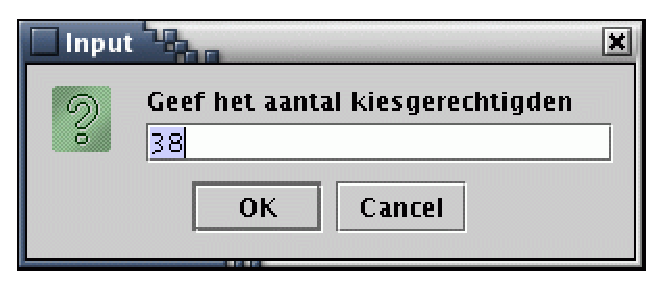
\includegraphics[scale=0.45]{scherm15}
\else
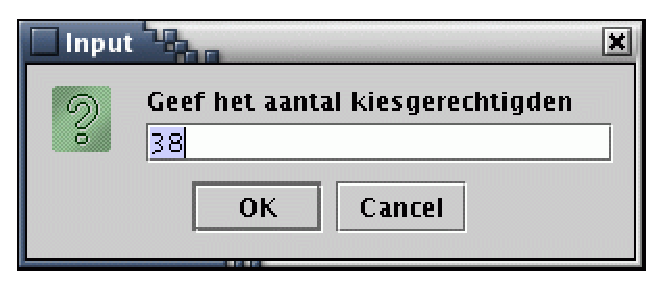
\includegraphics[scale=0.45]{scherm15.eps}
\fi
\caption{\rapport\ kiesgerechtigden}
\label{fig:rapport5}
\end{center}
\end{figure}
Uiteraard is het de verwachting dat het in te voeren getal duidelijk hoger zal zijn dan het aantal ingelezen stemmen, daar de opkomst meestal geen 100\% is.
Na het invoeren van een correct aantal, wordt het PDF bestand aangemaakt. Dit kan even duren.
\begin{figure}[b]
\begin{center}
\ifpdf
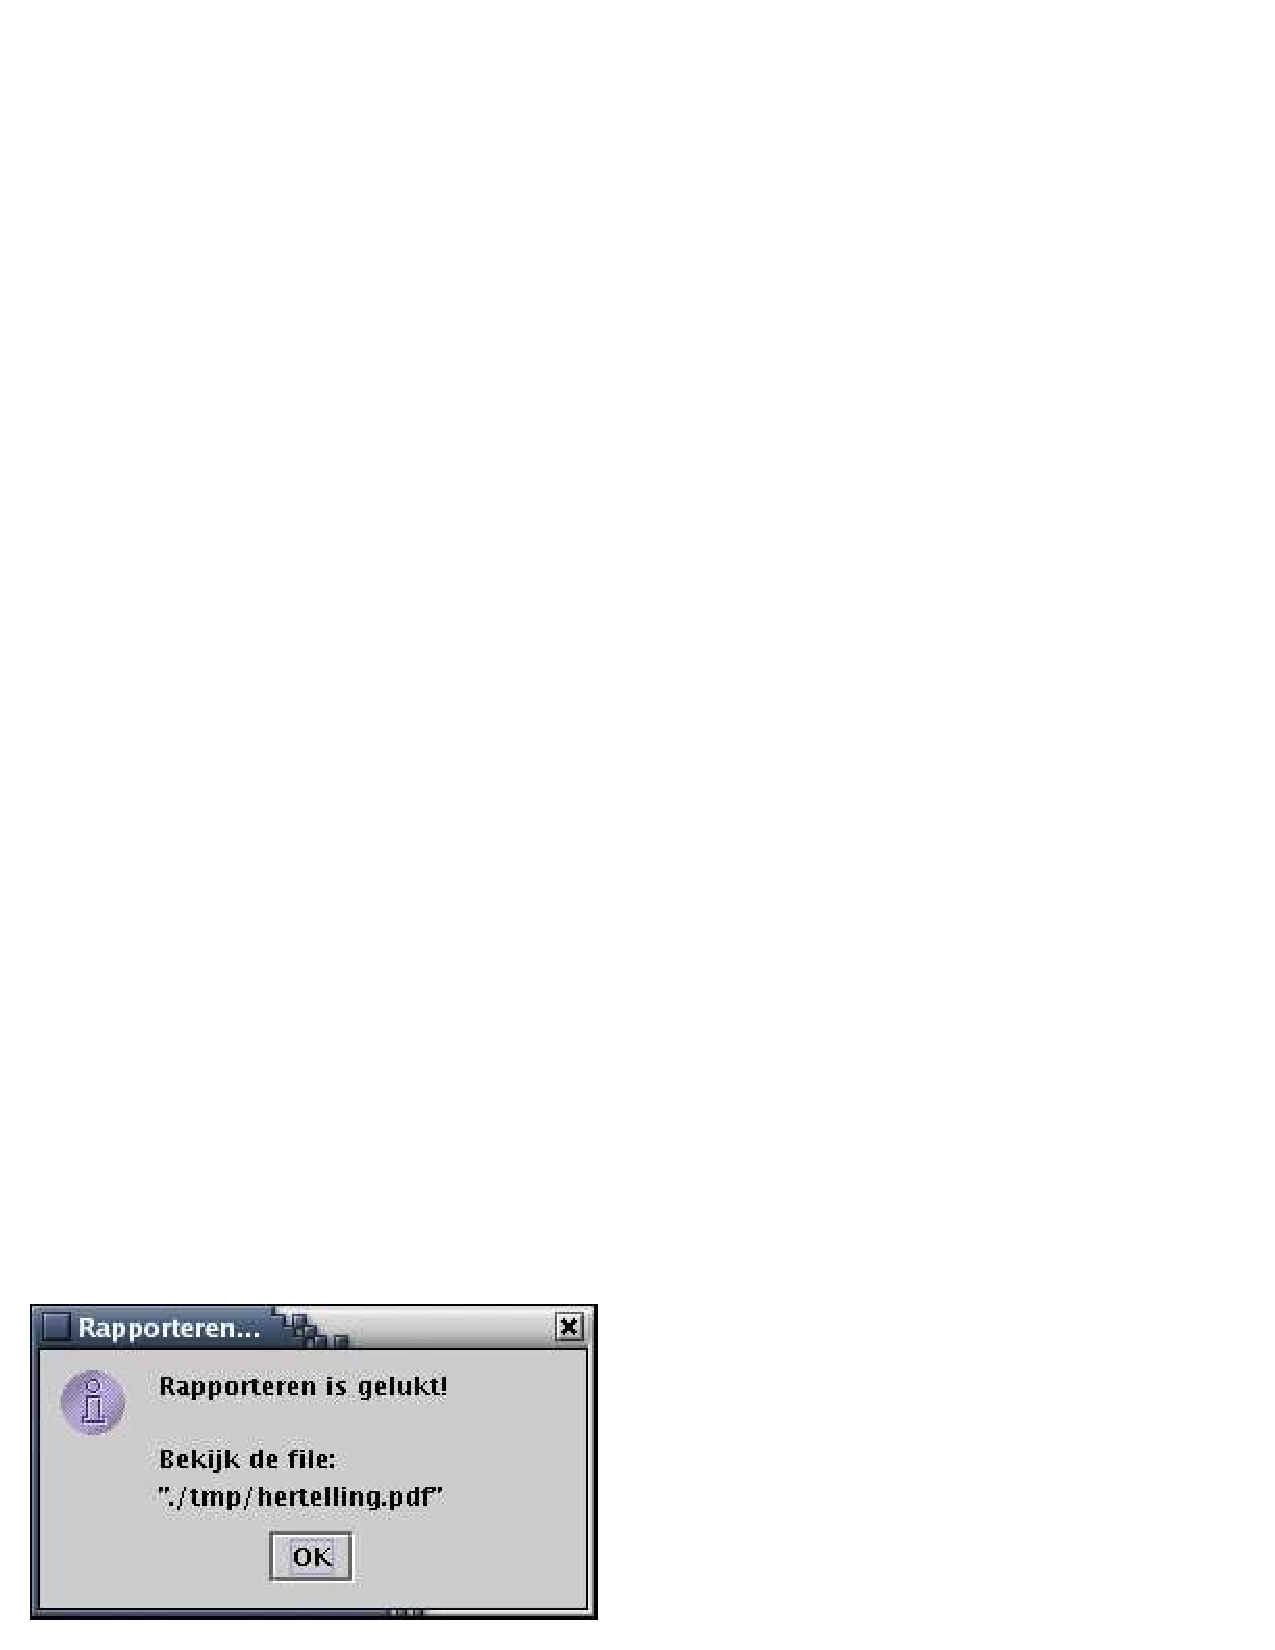
\includegraphics[scale=0.45]{scherm16}
\else
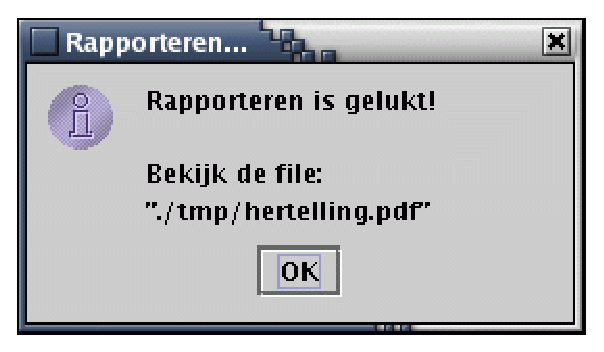
\includegraphics[scale=0.45]{scherm16.eps}
\fi
\caption{\rapport\ \resultaat}
\label{fig:rapport6}
\end{center}
\end{figure}
\begin{figure}[htb]
\begin{center}
\ifpdf
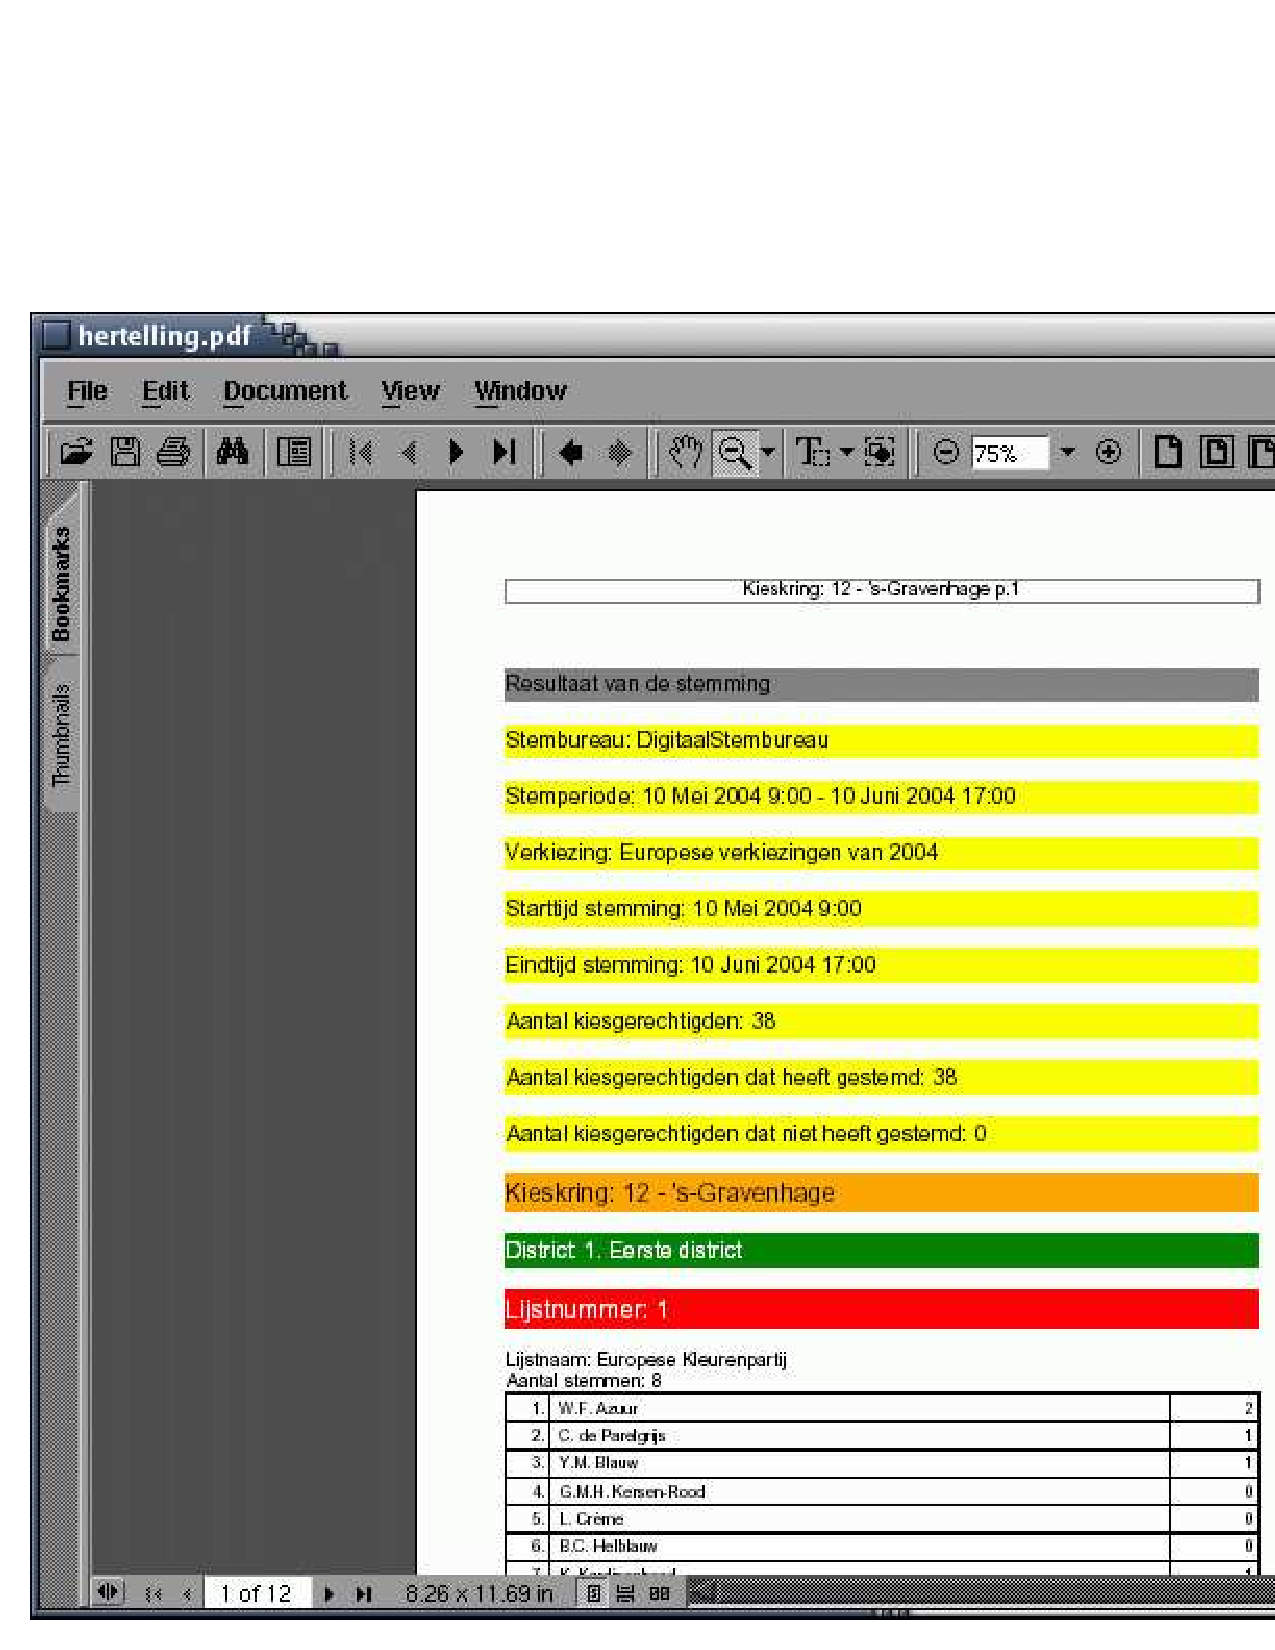
\includegraphics[scale=0.45]{scherm17}
\else
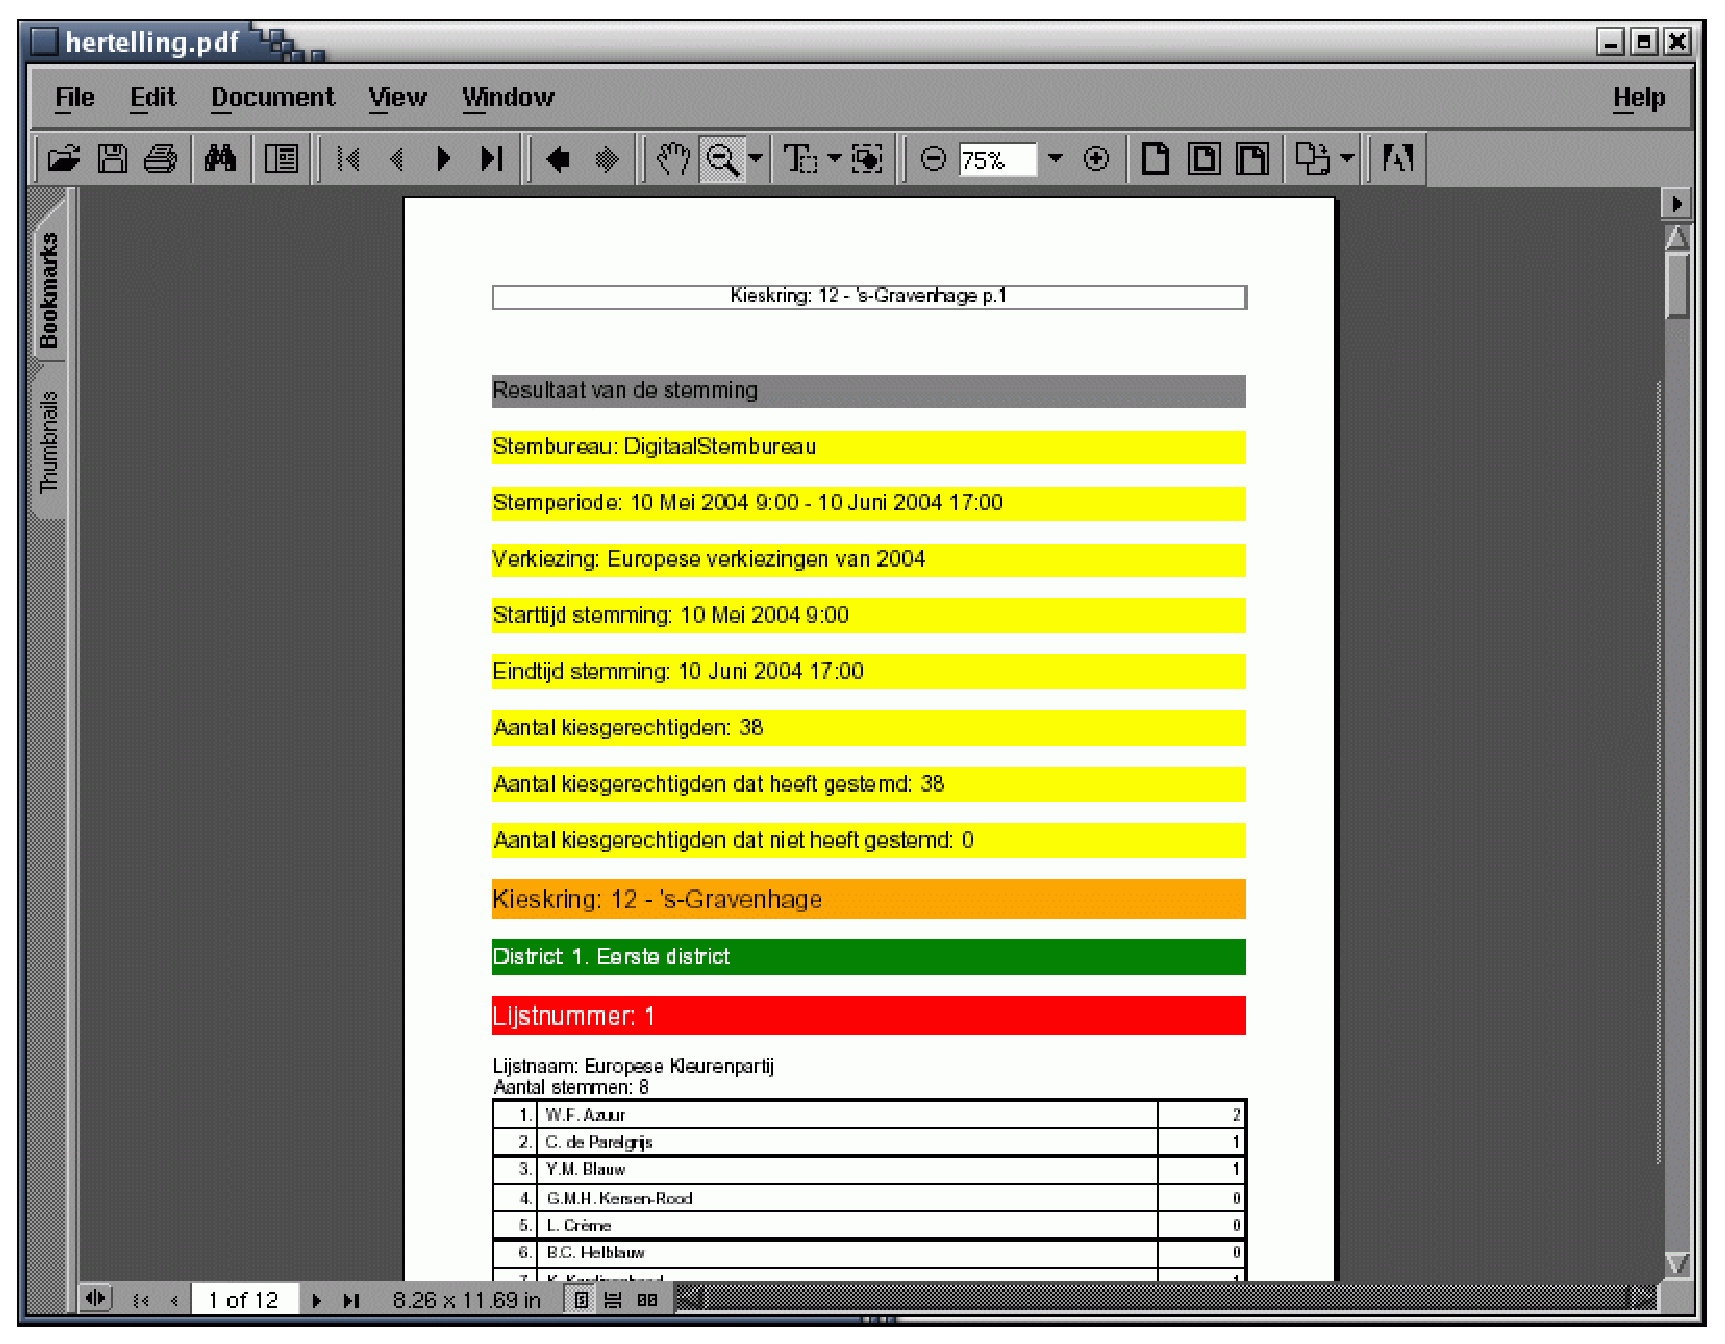
\includegraphics[scale=0.45]{scherm17.eps}
\fi
\caption{\rapport\ \resultaat}
\label{fig:rapport7}
\end{center}
\end{figure}
Evenals bij `\verwerking' wordt het bestand opgeslagen op schijf en indien mogelijk direct getoond op het scherm.

Na het succesvol aanmaken van een rapport, kan men vervolgens nog een keer kiezen voor `\rapport' om het andere rapport te maken.
\subsection{\help}
De beschikbaarheid is onafhankelijk van de toestand van het proces. Vandaar dat deze knop ook op een aparte plaats staat. Er wordt telkens een tekst getoond die specifiek uitlegt wat er op dat moment allemaal nog gedaan kan worden. Zie figuur~\ref{fig:help}.
\begin{figure}[htb]
\begin{center}
\ifpdf
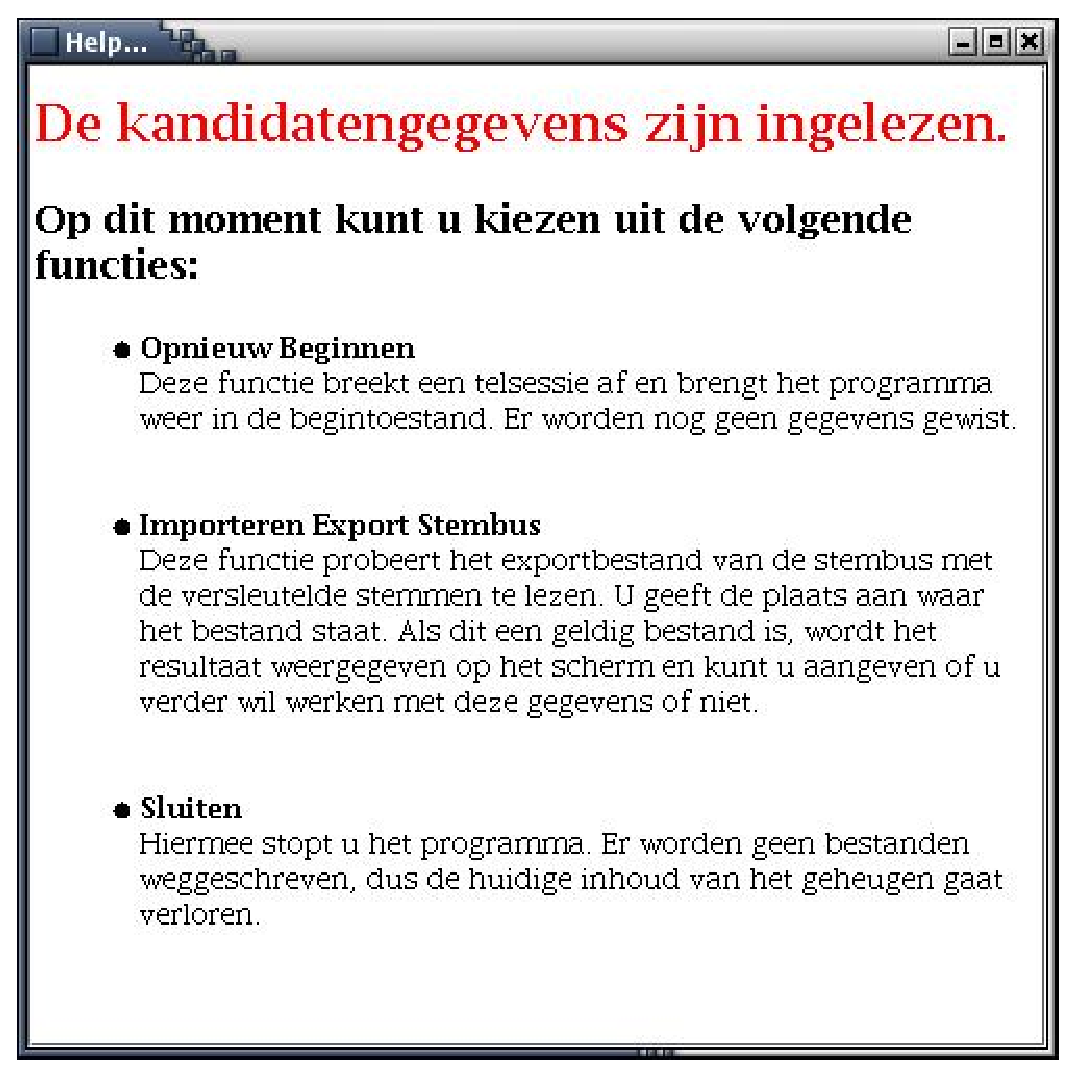
\includegraphics[scale=0.45]{scherm24}
\else
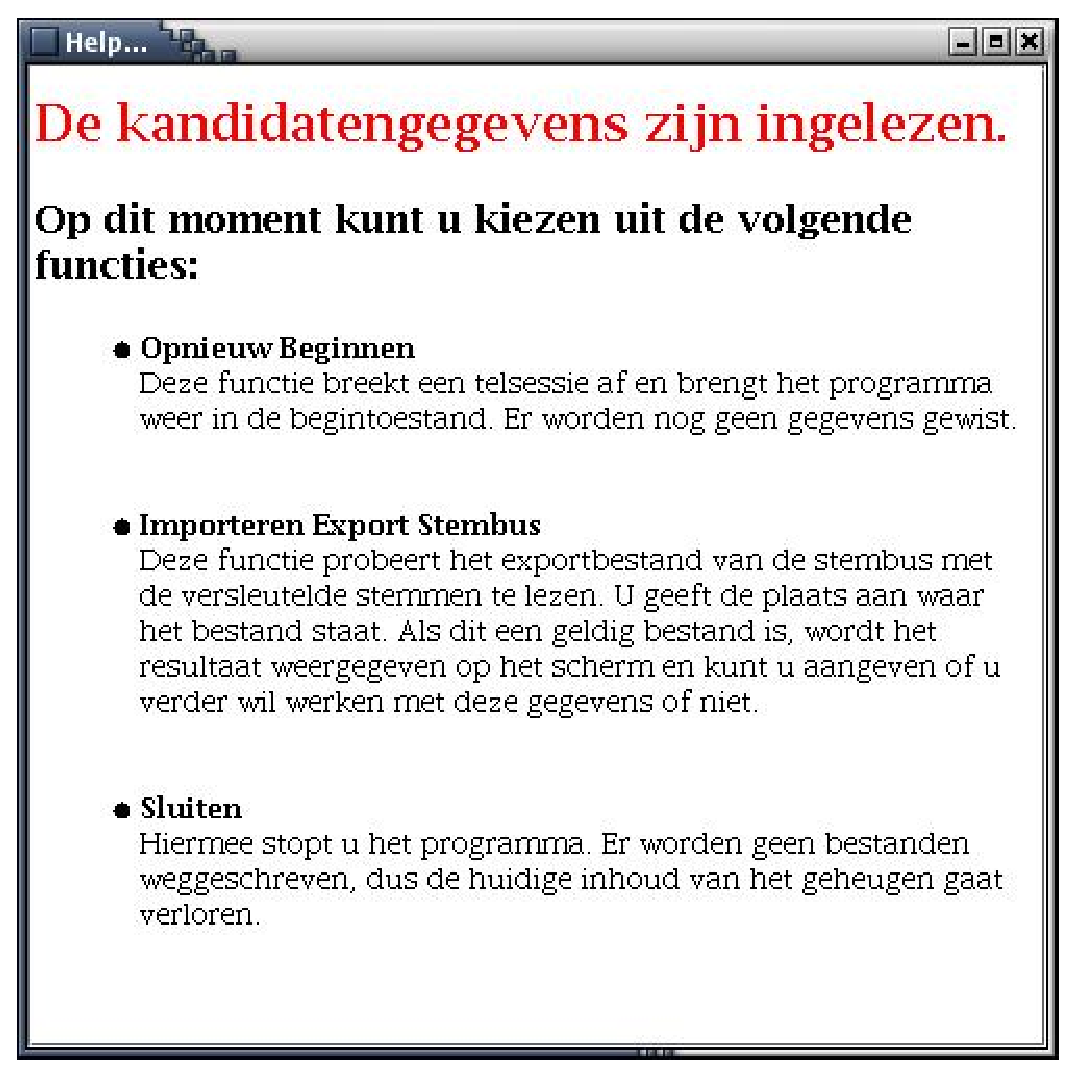
\includegraphics[scale=0.45]{scherm24.eps}
\fi
\caption{\help}
\label{fig:help}
\end{center}
\end{figure}
Als dit window niet gesloten wordt, zal de inhoud zich automatisch aanpassen
aan de uitgevoerde acties.
\subsection{\sluit}
Ook deze functie is altijd beschikbaar en sluit het programma af.
Hierbij wordt eerst om een bevestiging gevraagd. Zie figuur~\ref{fig:sluit}.
Gegevens in het geheugen worden uiteraard gewist bij het afsluiten. De PDF rapporten die op schijf zijn opgeslagen worden niet gewist en blijven dus beschikbaar.
Bij een volgende `run' van het programma zullen deze PDF bestanden gewist worden bij de optie `\wissen', maar ook dan zal er eerst nog om een bevestiging worden gevraagd.
\begin{figure}[htb]
\begin{center}
\ifpdf

\includegraphics[scale=0.45]{scherm20}
\else

\includegraphics[scale=0.45]{scherm20.eps}
\fi
\caption{\sluit}
\label{fig:sluit}
\end{center}
\end{figure}

\clearpage
\section{Contact}
Voor vragen over deze programmatuur, neem contact op met:
\begin{quote}
Engelbert Hubbers\\
Security of Systems groep\\
Katholieke Universiteit Nijmegen\\
Postbus 9010\\
6500 GL Nijmegen\\
\texttt{hubbers@cs.kun.nl}\\
+31 24 3652713\\
\url{http:www.cs.kun.nl/sos/}
\end{quote}
\bibliographystyle{plain}
\bibliography{usermanual}
\clearpage
\appendix
\section{Afwijkingen}\label{sec:afwijk}
Op sommige plaatsen wijkt ons programma af van de oorspronkelijke documentatie
in \cite{PVEBZK} en \cite{KOALOG}. Meestal is dit in overleg met BZK gebeurd;
soms puur op eigen initiatief als het om eenvoudige zaken gaat.
In deze sectie geven we een overzicht van deze punten.
\begin{enumerate}
\item De teksten in het hoofdmenu zijn zo gemaakt dat er bij alle acties een werkwoord staat. De helpfunctionaliteit wordt niet als actie gezien.
\item Er is een knop `\opnieuw' toegevoegd. Dit omdat \cite{PVEBZK} niet voorzag in de optie om een lopende sessie te onderbreken en opnieuw te beginnen.
\item Bij `\importkan' wordt in \cite{PVEBZK} alleen gevraagd om het aantal kandidaten per lijst. Omdat de naam van de lijst op dat moment toch al bekend is, tonen wij hier ook die naam.
\item Bij `\importkan' wordt gevraagd om een lijst op het scherm te krijgen met alle kandidaten en hun codes. Daar er rekening gehouden moet worden met 1000 codes per kandidaat wordt dit een enorm grote lijst. Daarom worden nu niet de codes genoemd maar alleen de kandidaten.
\item De optie van het importeren van sleutels is in ons programma expliciet opgesplitst in de keuze voor `\importpriv' en `\importpub'. De reden hiervoor is dat het nu voor de gebruiker duidelijker moet zijn welk type sleutelbestand geselecteerd moet worden. Omdat er na het succesvol importeren van een private sleutel geen extra informatie op het scherm getoond wordt, kan de gebruiker verbaasd raken door de tweede filebrowser voor de publieke sleutel.
De expliciete splitsing voorkomt dit probleem.
\item Het aangeleverde testbestand met de kandidaatcodes was niet geldig ten opzichte van de DTD in \cite{KOALOG}. Afgezien van het probleem met de `\relax"\relax' bij `Partij van de "sport"', bleek ook dat het geslacht niet altijd `M' of `V' was zoals vereist in de DTD. Daarnaast beschikt de DTD niet over het veld `codecount' terwijl dat wel in de file staat.
Hierom hebben wij besloten niet strikt die DTD te gebruiken, maar een iets soepelere versie.
\item Ook het stembusbestand voldeed niet aan de DTD in \cite{KOALOG}. Dit had te maken met de hoofdletters. Wij gebruiken hier dan ook niet de gegeven DTD maar de versie die werkt met het testbestand.
\item In het verwerkingsverslag wordt volgens de definitie het referentienummer van het kandidatenbestand getoond. Daar het niet geheel duidelijk is of het hier om de `request' dan wel `response' referentie gaat, tonen wij beide.
\item
In het verwerkingsverslag hebben we bij alle files waar om een timestamp wordt gevraagd, gezorgd dat de begeleidende tekst hetzelfde was. Dat is in \cite{PVEBZK} niet het geval.
\item In het eindverslag met het resultaat van de stemming wijken wij ook af van de definitie in \cite{PVEBZK}. In de definitie staat namelijk dat de regel voor aantal stemmen leeg moet blijven om later met de hand in te vullen. Wij hebben dit opgelost door bij het aanmaken van dit rapport de gebruiker dit aantal stemgerechtigden in te laten voeren. Motivatie hiervoor is dat in het ons ter beschikking gestelde voorbeeldbestand dit getal ook al is ingevuld.
\item Verder bevat het voorbeeldrapport dat wij gekregen hebben ook een regel voor het aantal kiesgerechtigden dat niet gestemd heeft die niet in de definitie staat. Wij hebben ook zo'n regel opgenomen waarbij de waarde van dit veld wordt bepaald door het aantal getelde stemmen af te trekken van het ingevoerde aantal kiesgerechtigden.
\item Ons verslag gebruikt kleuren om duidelijk onderscheid te kunnen maken tussen globale informatie als het stembureau en de periode en de informatie per kieskring. Omdat er bij deze vekiezingen slechts \'e\'en kieskring gebruikt wordt, is de toegevoegde waarde niet echt groot.
\item In het bijzonder is dit ook de reden waarom de regel met `Kieskring' pas onder de globale informatie staat. Dit om voorbereid te zijn op invoer met meerdere kieskringen.
%\item Om voorbereid te zijn op een uitbreiding wordt ook het district op ons verslag genoemd.
\item Op speciaal verzoek schrijven wij een file \texttt{tmp/decrypted.txt} weg met daarin de ontsleutelde stemmen. Deze file wordt niet gewist na het afsluiten van het programma. Hij wordt wel automatisch gewist bij de functie `\wissen'.
\end{enumerate}
\end{document}
